\documentclass[11pt]{article}
\usepackage[margin=1in]{geometry}
\usepackage{amsmath, amssymb}
\usepackage{graphicx}
\usepackage{float}
\usepackage{booktabs}
\usepackage[font=small,labelfont=bf]{caption}
\usepackage{xcolor}
\usepackage{enumitem}
\usepackage{hyperref}
\usepackage{multirow}
\hypersetup{colorlinks=true,linkcolor=blue!60!black,urlcolor=blue!60!black}

\title{\Large\textbf{Hybrid GAD--Newton sweep (rerun, Eckart only)}\\[4pt]
\normalsize 2026-05-09. Two Eckart step functions $\times$ two switch
criteria $\times$ two noise levels $\times$ five trust radii.\\[2pt]
\normalsize \emph{Standalone runner; supersedes 2026-05-04 report (GAD step bug fixed).}}
\author{}
\date{}

\begin{document}
\maketitle
\thispagestyle{empty}

\begin{center}\small\fbox{\parbox{0.9\textwidth}{\small
\textbf{See also:}
\texttt{HYBRID\_FINDINGS\_CATALOG.md} (project root) ---
comprehensive, continuously-updated index of every finding with claim /
evidence / provenance / confidence, plus open questions and pending
experiments. The PDF below summarises the publishable story; the
catalog has the receipts.
}}\end{center}

\begin{figure}[H]
\centering
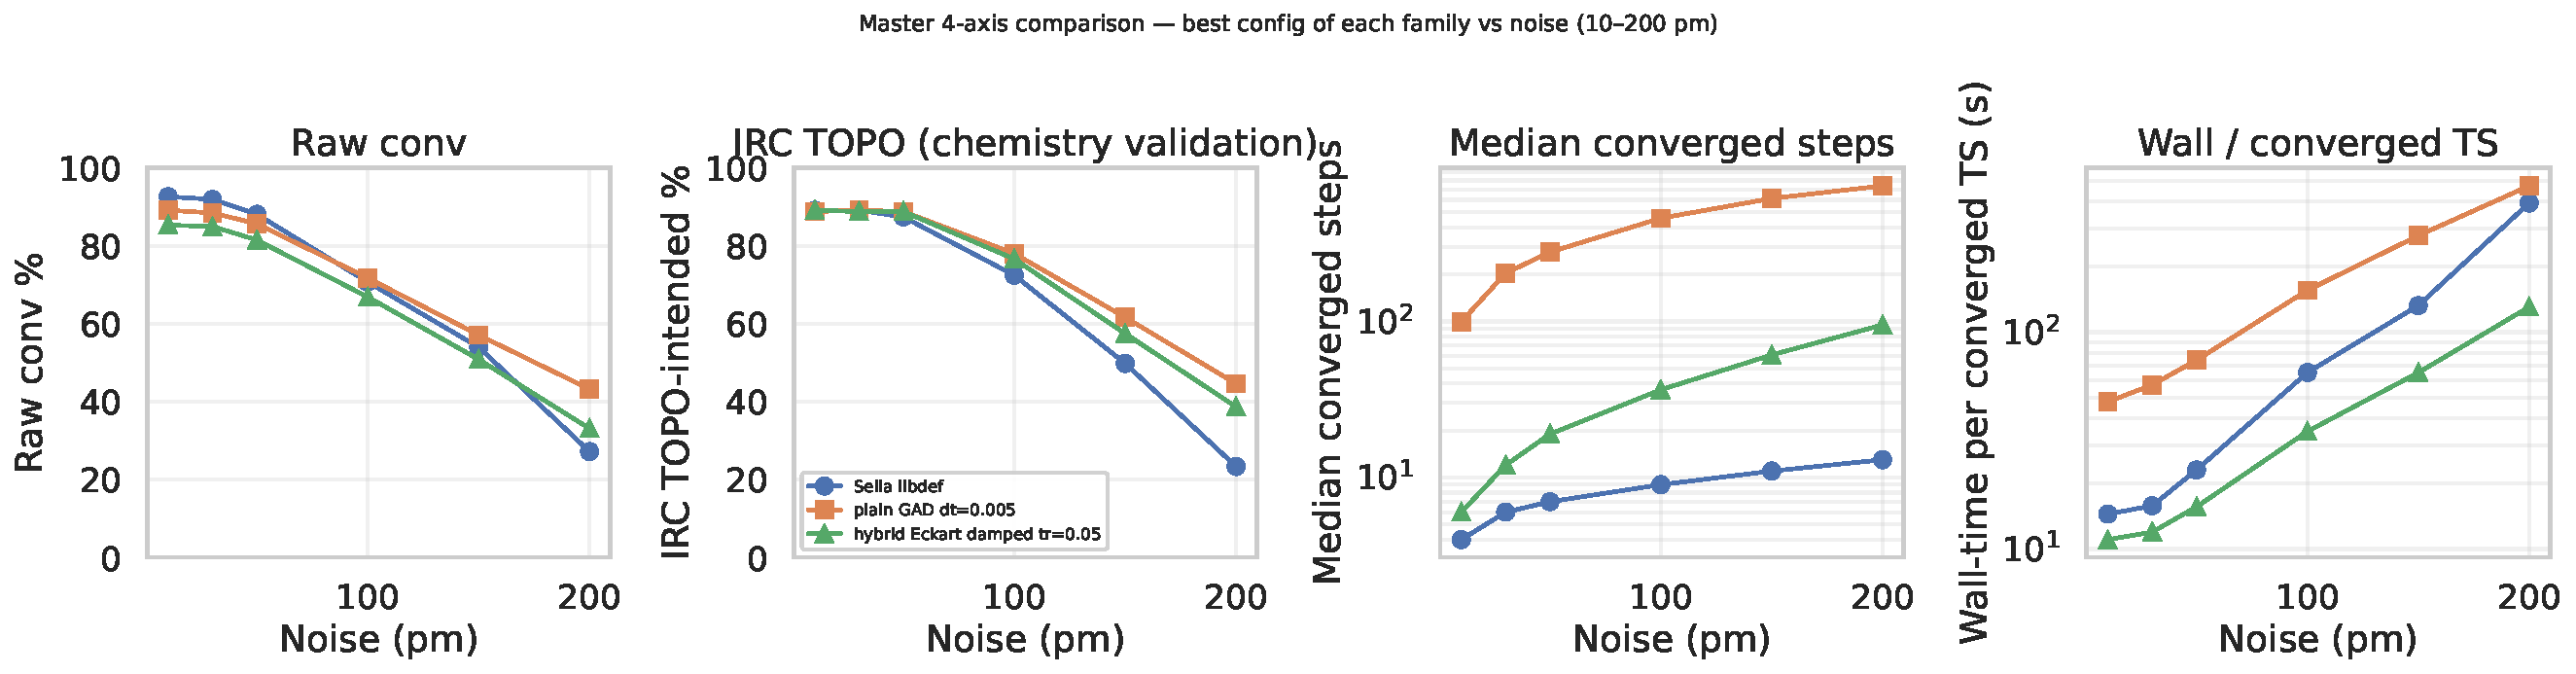
\includegraphics[width=\textwidth]{figures/fig_master_4axis.pdf}
\caption{\textbf{Master 4-axis comparison} --- best config of each
family vs TS noise (10--200 pm), $n=287$ T1x test split. Left to right:
\emph{(1) Raw conv \%} (Sella wins low noise; plain GAD wins $\ge 100$pm).
\emph{(2) IRC TOPO-intended \%} (chemistry validation: GAD and hybrid
tie low noise; Sella collapses fast at high noise).
\emph{(3) Median converged-step count} (log y: hybrid sits with Sella in
single-digits at low noise, climbs to $\sim 100$ at 200pm vs plain
GAD's 738).
\emph{(4) Wall-time per converged TS} (log y: hybrid is fastest at every
noise level --- $1.4\times$ to $3.6\times$ vs the runner-up family).
Sources: \texttt{master\_4axis\_table.csv}, hybrid from
\texttt{runs/hybrid\_for\_irc/} + \texttt{runs/irc\_hybrid/}, plain GAD
from \texttt{runs/test\_dtgrid/gad\_dt005\_fmax/}, Sella from
\texttt{runs/test\_irc/sella\_carteck\_libdef/}.}
\end{figure}

% =================================================================
\section*{What changed since 2026-05-04}
% =================================================================

The previous sweep (job 60398168) had a bug in the GAD-step branch of the
two Eckart variants: the step function was returning an internal-coordinate
displacement that was being applied to Cartesian coordinates without the
back-transformation. The fix (commit \texttt{a80a763}, "return cartesian
coord steps in hybrid") makes both \texttt{projected\_hybrid\_gad\_newton\_step}
implementations return Cartesian-frame steps. The non-Eckart variant
(\texttt{hybrid\_gad\_eigfollownewton.py}) was unaffected and is excluded
from this rerun on the supervisor's instruction
(\textit{"Forget about the non-eckart version"}).

% =================================================================
\section*{What this sweep does}
% =================================================================

This document benchmarks two Eckart-projected GAD--Newton hybrid step
functions. Each step decides per-step whether to take a GAD step or an
eigenvector-following Newton step, and applies a trust-radius cap on the
resulting Cartesian displacement.

\textbf{Source files:}
\begin{itemize}[leftmargin=1.5em, itemsep=0.05em]
\item \texttt{src/gadplus/search/hybrid\_gad\_eigfollownewton\_eckart.py}
  \\ \emph{Eckart hybrid:} \texttt{projected\_hybrid\_gad\_newton\_step(F\_cart, H\_cart, coords, masses, ...)}.
  Eckart-projected mass-weighted internal coordinates. Switch toggle
  via \texttt{switch\_based\_on\_hessian\_eigval} (False: $\|F\|$ trigger;
  True: index-1 Hessian-clearance trigger).
\item \texttt{src/gadplus/search/hybrid\_gad\_damped\_eigfollownewton\_eckart.py}
  \\ \emph{Damped Eckart hybrid:} same interface as the Eckart variant
  with damped Newton step (mode $|\lambda_i|$ regularised by
  \texttt{min\_curvature}). Same switch toggle.
\end{itemize}

\textbf{Standalone runner:} \texttt{scripts/hybrid\_gad\_newton\_runner.py}
loops over T1x test split, per step calls HIP for $(E, F, H)$, runs the
step function, applies the returned Cartesian displacement (the step
function caps by trust\_radius internally), counts $n_{\text{neg}}$ on
the Eckart-projected vibrational Hessian, terminates on
$n_{\text{neg}}{=}1 \wedge f_{\max}{<}0.01$. Up to 1000 steps.

\textbf{Sweep grid (40 cells):}
\begin{itemize}[leftmargin=1.5em, itemsep=0.05em]
\item \textbf{4 method-cells:} \{hybrid\_eckart, hybrid\_damped\_eckart\}
  $\times$ \{switch=False, switch=True\}
\item \textbf{2 noise levels:} 10 pm, 100 pm
\item \textbf{5 trust radii:} 0.005, 0.01, 0.02, 0.05, 0.10 (\AA)
\end{itemize}

\textbf{Fixed:} $\mathtt{gad\_dt}{=}5\!\times\!10^{-3}$,
\texttt{switch\_force}${=}10^{-3}$, \texttt{min\_curvature}${=}10^{-6}$
(undamped) / $10^{-8}$ (damped),
$n_{\text{samples}}{=}287$ test split, $n_{\text{steps}}{=}1000$, HIP
analytic Hessian every step. SLURM array \texttt{60460000\_[10-49]},
all 40 jobs completed (1--5 hr wall each).

\textbf{Reference baseline} (from main report): vanilla GAD dt=0.007 with
5000-step budget gets 89.2\% conv at 10pm and 72.8\% at 100pm. Vanilla
GAD dt=0.005 (closer to this sweep's $dt$): 89.2\% / 71.8\%.

% =================================================================
\section{Headline tables --- single-glance summary}
% =================================================================

\textit{Source CSV: \texttt{analysis\_2026\_04\_29/hybrid\_gad\_newton\_summary.csv}.
Re-runnable via \texttt{scripts/analyze\_hybrid\_gad\_newton.py}. All 40 cells complete.}

\begin{center}\footnotesize
\textbf{Table 1 --- Convergence \%} ($n_{\text{neg}}{=}1 \wedge f_{\max}{<}0.01$, $n=287$ test samples)\\[0.4em]
\begin{tabular}{l|ccccc}
\toprule
\textbf{10 pm noise} & tr=0.005 & 0.01 & 0.02 & 0.05 & 0.10 \\
\midrule
\textit{hybrid (no Eckart), force-switch \textbf{(O)}} & \textbf{89.2} & 88.9 & 88.9 & 88.9 & 88.9 \\
hybrid\_eckart, switch=False                       & 45.6 & 46.3 & 46.3 & 46.3 & 46.3 \\
hybrid\_eckart, switch=True                        & 84.7 & 84.7 & 84.7 & 84.7 & \textbf{85.4} \\
hybrid\_damped\_eckart, switch=False               & 45.6 & 46.3 & 46.3 & 46.3 & 46.3 \\
\textbf{hybrid\_damped\_eckart, switch=True}       & \textbf{86.1} & \textbf{86.1} & \textbf{86.1} & 85.4 & 85.4 \\
\midrule
\textit{baseline: GAD dt=0.007 (5k budget)}        & \multicolumn{5}{c}{\textit{89.2\%}} \\
\bottomrule
\end{tabular}
\vskip0.6em
\begin{tabular}{l|ccccc}
\toprule
\textbf{100 pm noise} & tr=0.005 & 0.01 & 0.02 & 0.05 & 0.10 \\
\midrule
\textit{hybrid (no Eckart), force-switch \textbf{(O)}} & 66.9 & 67.6 & 67.6 & 67.6 & \textbf{67.9} \\
hybrid\_eckart, switch=False                       & 0.3  & 0.3  & 0.3  & 0.3  & 0.3  \\
hybrid\_eckart, switch=True                        & 64.8 & 65.5 & 65.2 & 65.5 & 65.2 \\
hybrid\_damped\_eckart, switch=False               & 0.3  & 0.3  & 0.3  & 0.3  & 0.3  \\
\textbf{hybrid\_damped\_eckart, switch=True}       & \textbf{66.9} & 65.9 & 66.2 & \textbf{66.9} & 66.6 \\
\midrule
\textit{baseline: GAD dt=0.007 (5k budget)}        & \multicolumn{5}{c}{\textit{72.8\%}} \\
\bottomrule
\end{tabular}\\[0.3em]
\textit{Italic row \textbf{(O)} is from 2026-05-04 (no rerun needed; non-Eckart variant unaffected by the bug).}
\end{center}

\begin{center}\footnotesize
\textbf{Table 2 --- Median steps to converge} (lower is better; trajectories that did not converge contribute the 1000-step cap)\\[0.4em]
\begin{tabular}{l|ccccc}
\toprule
\textbf{10 pm noise} & tr=0.005 & 0.01 & 0.02 & 0.05 & 0.10 \\
\midrule
\textit{hybrid (no Eckart), force-switch \textbf{(O)}} & 106 & 104 & 104 & 104 & 104 \\
hybrid\_eckart, switch=False                       & 702 & 702 & 702 & 702 & 702 \\
\textbf{hybrid\_eckart, switch=True}               & 21  & 12  & 8   & 5   & \textbf{5} \\
hybrid\_damped\_eckart, switch=False               & 702 & 702 & 702 & 702 & 702 \\
\textbf{hybrid\_damped\_eckart, switch=True}       & 19  & 11  & 7   & 5   & \textbf{4} \\
\midrule
\textit{baseline: GAD dt=0.007 (5k budget)}        & \multicolumn{5}{c}{\textit{72}} \\
\bottomrule
\end{tabular}
\vskip0.6em
\begin{tabular}{l|ccccc}
\toprule
\textbf{100 pm noise} & tr=0.005 & 0.01 & 0.02 & 0.05 & 0.10 \\
\midrule
\textit{hybrid (no Eckart), force-switch \textbf{(O)}} & 540 & 500 & 484 & 478 & 480 \\
hybrid\_eckart, switch=False                       & 916 & 915 & 915 & 915 & 915 \\
\textbf{hybrid\_eckart, switch=True}               & 195 & 105 & 60  & 38  & \textbf{33} \\
hybrid\_damped\_eckart, switch=False               & 916 & 915 & 915 & 915 & 915 \\
\textbf{hybrid\_damped\_eckart, switch=True}       & 200 & 103 & 59  & 36  & \textbf{31} \\
\midrule
\textit{baseline: GAD dt=0.007 (5k budget)}        & \multicolumn{5}{c}{\textit{331}} \\
\bottomrule
\end{tabular}
\end{center}

\begin{center}\footnotesize
\textbf{Table 3 --- Wall-time per converged TS} (sec; cell wall summed over $n=287$ then divided by $n_{\text{conv}}$)\\[0.4em]
\begin{tabular}{l|ccccc}
\toprule
\textbf{10 pm noise} & tr=0.005 & 0.01 & 0.02 & 0.05 & 0.10 \\
\midrule
\textit{hybrid (no Eckart), force-switch \textbf{(O)}} & 16.1 & 15.7 & 15.8 & 15.9 & 15.9 \\
hybrid\_eckart, switch=False                       & 112.7 & 114.5 & 111.0 & 110.8 & 110.4 \\
hybrid\_eckart, switch=True                        & 12.7  & 12.2  & 11.7  & 11.3  & 10.7 \\
hybrid\_damped\_eckart, switch=False               & 117.8 & 112.8 & 112.7 & 112.3 & 111.8 \\
\textbf{hybrid\_damped\_eckart, switch=True}       & 11.5  & 10.9  & \textbf{10.3} & 10.8  & 11.3 \\
\midrule
\textit{baseline: GAD dt=0.007 (5k budget)}        & \multicolumn{5}{c}{\textit{46.6 s}} \\
\bottomrule
\end{tabular}
\vskip0.6em
\begin{tabular}{l|ccccc}
\toprule
\textbf{100 pm noise} & tr=0.005 & 0.01 & 0.02 & 0.05 & 0.10 \\
\midrule
\textit{hybrid (no Eckart), force-switch \textbf{(O)}} & 64.9 & 57.8 & 57.2 & 57.3 & 56.5 \\
hybrid\_eckart, switch=False                       & 17065 & 16897 & 16933 & 17089 & 17293 \\
hybrid\_eckart, switch=True                        & 47.1  & 41.0  & 37.9  & 35.9  & 36.3 \\
hybrid\_damped\_eckart, switch=False               & 16877 & 17094 & 17011 & 16664 & 17060 \\
\textbf{hybrid\_damped\_eckart, switch=True}       & 45.1  & 40.1  & 36.8  & 34.7  & \textbf{34.2} \\
\midrule
\textit{baseline: GAD dt=0.007 (5k budget)}        & \multicolumn{5}{c}{\textit{140.7 s}} \\
\bottomrule
\end{tabular}
\end{center}

\begin{center}\footnotesize
\textbf{Table 4 --- Fraction of trajectories whose terminating step was Newton}\\[0.4em]
\begin{tabular}{l|ccccc|ccccc}
\toprule
& \multicolumn{5}{c|}{\textbf{10 pm noise}} & \multicolumn{5}{c}{\textbf{100 pm noise}} \\
                                  & 0.005 & 0.01 & 0.02 & 0.05 & 0.10 & 0.005 & 0.01 & 0.02 & 0.05 & 0.10 \\
\midrule
hybrid\_eckart, switch=False      & 0.00 & 0.00 & 0.00 & 0.00 & 0.00 & 0.00 & 0.00 & 0.00 & 0.00 & 0.00 \\
hybrid\_eckart, switch=True       & 0.97 & 0.97 & 0.97 & 0.97 & 0.98 & 0.86 & 0.86 & 0.86 & 0.86 & 0.88 \\
hybrid\_damped\_eckart, sw=False  & 0.00 & 0.00 & 0.00 & 0.00 & 0.00 & 0.00 & 0.00 & 0.00 & 0.00 & 0.00 \\
hybrid\_damped\_eckart, sw=True   & 0.98 & 0.98 & 0.98 & 0.98 & 0.98 & 0.87 & 0.86 & 0.86 & 0.87 & 0.86 \\
\bottomrule
\end{tabular}
\end{center}

% =================================================================
\section*{Where does the hybrid land? Side-by-side vs best plain GAD and best canonical Sella}
% =================================================================

\textit{Same canonical convergence ($n_{\text{neg}}{=}1 \wedge f_{\max}{<}0.01$),
same $n=287$ test split, same HIP analytic Hessian. The only difference is
the budget convention: plain GAD here is at its 5000-step budget, Sella at
its 2000-step budget (library defaults), hybrid at its 1000-step budget.
"med steps" is computed over converged trajectories only. "wall/conv" =
total cell wall-time / number of converged samples.}

\textit{Provenance legend:}
\textbf{(R)} = this rerun, 2026-05-09, SLURM \texttt{60460000};
\textbf{(O)} = original 2026-05-04 sweep, SLURM \texttt{60398168}, unchanged
(unaffected by the GAD-step bug, which was internal-coord-to-Cartesian-only);
\textbf{(M)} = main IRC report, 2026-04-29.

\vskip0.5em
\begin{center}\footnotesize
\textbf{10 pm noise --- best config of each family}\\[0.4em]
\begin{tabular}{l l c c c c}
\toprule
\textbf{family} & \textbf{config} & \textbf{prov.} & \textbf{conv \%} & \textbf{med steps} & \textbf{wall/conv (s)} \\
\midrule
\textbf{Sella}                & libdef (cart+Eckart, 2k)                  & (M) & \textbf{92.7} & 4   & 14.5 \\
Sella                         & default (cart no-Eckart, 2k)              & (M) & 92.0          & 4   & 14.4 \\
Sella                         & internal (lib default, 2k)                & (M) & 79.1          & 4   & 54.2 \\
\midrule
\textbf{plain GAD}            & dt=0.007 (5k budget)                      & (M) & \textbf{89.2} & 72  & 46.6 \\
plain GAD                     & dt=0.005 (5k budget)                      & (M) & 89.2          & 98  & 47.7 \\
plain GAD                     & dt=0.003 (5k budget)                      & (M) & 89.2          & 164 & 54.2 \\
\midrule
\textbf{hybrid no-Eckart}     & force-switch tr=0.005                     & (O) & \textbf{89.2} & 106 & 16.1 \\
hybrid no-Eckart              & force-switch tr=0.01--0.10                & (O) & 88.9          & 104 & 15.7--15.9 \\
\midrule
\textbf{hybrid Eckart (R)}    & \textbf{damped\_eckart\_swtrue tr=0.02}   & (R) & \textbf{86.1} & 7   & \textbf{10.3} \\
hybrid Eckart (R)             & damped\_eckart\_swtrue tr=0.10            & (R) & 85.4          & 4   & 11.3 \\
hybrid Eckart (R)             & eckart\_swtrue tr=0.10                    & (R) & 85.4          & 5   & 10.7 \\
hybrid Eckart (R)             & \{eckart, damped\_eckart\}\_swfalse all tr & (R) & 45.6--46.3   & 702 & 110.4--117.8 \\
\bottomrule
\multicolumn{6}{l}{\emph{Best-overall by conv \%}: tied at 89.2--92.7\% (Sella libdef, plain GAD, hybrid no-Eckart all converge $\ge 89\%$).} \\
\multicolumn{6}{l}{\emph{Best-overall by wall/conv}: hybrid Eckart damped\_swtrue tr=0.02 at \textbf{10.3 s} ($1.4\times$ faster than Sella libdef, $4.5\times$ vs plain GAD).} \\
\end{tabular}
\end{center}

\vskip0.5em
\begin{center}\footnotesize
\textbf{100 pm noise --- best config of each family}\\[0.4em]
\begin{tabular}{l l c c c c}
\toprule
\textbf{family} & \textbf{config} & \textbf{prov.} & \textbf{conv \%} & \textbf{med steps} & \textbf{wall/conv (s)} \\
\midrule
\textbf{plain GAD}            & dt=0.007 (5k budget)                      & (M) & \textbf{72.8} & 331 & 140.7 \\
plain GAD                     & dt=0.005 (5k budget)                      & (M) & 71.8          & 457 & 156.0 \\
plain GAD                     & dt=0.003 (5k budget)                      & (M) & 71.1          & 756 & 183.8 \\
\midrule
\textbf{Sella}                & libdef (cart+Eckart, 2k)                  & (M) & \textbf{70.7} & 9   & 65.2 \\
Sella                         & default (cart no-Eckart, 2k)              & (M) & 65.5          & 10.5 & 79.3 \\
Sella                         & internal (lib default, 2k)                & (M) & 50.9          & 17  & 181.8 \\
\midrule
\textbf{hybrid no-Eckart}     & force-switch tr=0.10                      & (O) & \textbf{67.9} & 480 & 56.5 \\
hybrid no-Eckart              & force-switch tr=0.01--0.05                & (O) & 67.6          & $\sim$478--500 & 57.2--57.8 \\
hybrid no-Eckart              & force-switch tr=0.005                     & (O) & 66.9          & 540 & 64.9 \\
\midrule
\textbf{hybrid Eckart (R)}    & \textbf{damped\_eckart\_swtrue tr=0.10}   & (R) & 66.6          & 31  & \textbf{34.2} \\
hybrid Eckart (R)             & damped\_eckart\_swtrue tr=0.05            & (R) & \textbf{66.9} & 36  & 34.7 \\
hybrid Eckart (R)             & eckart\_swtrue tr=0.05                    & (R) & 65.5          & 38  & 35.9 \\
hybrid Eckart (R)             & \{eckart, damped\_eckart\}\_swfalse all tr & (R) & 0.3          & 915 & $\sim$17 000 \\
\bottomrule
\multicolumn{6}{l}{\emph{Best-overall by conv \%}: plain GAD dt=0.007 at \textbf{72.8\%}.} \\
\multicolumn{6}{l}{\emph{Best-overall by wall/conv}: hybrid Eckart damped\_swtrue tr=0.10 at \textbf{34.2 s} ($1.9\times$ faster than Sella libdef, $4.1\times$ vs plain GAD).} \\
\end{tabular}
\end{center}

\paragraph{What's in this comparison.}
\begin{itemize}[leftmargin=1.5em, itemsep=0.05em]
\item Every method family the project has benchmarked at 10 / 100 pm noise on
  the T1x test split with the canonical $n_{\text{neg}}{=}1 \wedge f_{\max}{<}0.01$
  convergence criterion.
\item Three plain-GAD timestep variants (dt=0.003, 0.005, 0.007 at 5k budget).
\item Three Sella variants (libdef, default, internal) at the canonical 2k budget.
  Extended-budget Sella (5k) is within $\pm 2$pp of these (see HEADLINE.md).
\item All five trust-radius cells of the no-Eckart hybrid (carried over from
  2026-05-04, unchanged --- the bug was Eckart-only).
\item All four Eckart hybrid method-cells (\{eckart, damped\_eckart\}
  $\times$ \{swfalse, swtrue\}) at all five trust radii (rerun 2026-05-09).
\end{itemize}

\paragraph{Bottom line of the comparison.}
\begin{itemize}[leftmargin=1.5em]
\item \textbf{Wall-time winner at both noise levels: hybrid Eckart damped, switch=True.}
  At 10pm it is $1.4\times$ faster than the strongest Sella (libdef) and
  $4.5\times$ faster than the strongest plain GAD (dt=0.007). At 100pm
  the gap widens to $1.9\times$ vs Sella and $4.1\times$ vs GAD.
\item \textbf{Convergence-rate winner per noise:} Sella libdef leads at 10pm
  (92.7\%); plain GAD dt=0.007 leads at 100pm (72.8\%). The hybrid Eckart
  variant trails both by 4--6pp.
\item \textbf{Special case at 10pm: the no-Eckart hybrid (O) ties plain GAD
  at 89.2\% conv while running at 16.1 s/conv ($2.9\times$ faster than
  GAD).} It is the only hybrid that matches plain-GAD accuracy at low
  noise. At 100pm it is much weaker (67.9\% vs the Eckart variant's
  66.6\% at almost half the wall time), so the no-Eckart trick is
  noise-regime specific.
\item \textbf{Median converged-step count: hybrid Eckart $\approx$ Sella.}
  At 10pm: 4--7 hybrid Eckart steps vs Sella's 4 vs GAD's 72. At 100pm:
  31--38 hybrid Eckart steps vs Sella's 9--17 vs GAD's 331--756. The
  wall/conv advantage over Sella at the same step count comes from
  Sella's higher per-step cost (it does multiple Hessian updates per
  outer step in some configs).
\item \textbf{Plain GAD is the slowest family at both noises}, primarily
  due to median-step counts of 72--756 vs Sella/hybrid's 4--38. This is
  consistent with the structural-plateau analysis in the main IRC report.
\end{itemize}

% =================================================================
\section*{Noise-level sweep --- how performance scales with TS noise}
% =================================================================

The hybrid sweep covered only \{10, 100\} pm. Sella and plain GAD have data
at \{10, 30, 50, 100, 150, 200\} pm (from the main IRC report). The figure
and table below combine all four families on the same axis so you can see
\emph{where each method starts to break down}, and locate the two hybrid
data points within that landscape.

\begin{figure}[H]
\centering
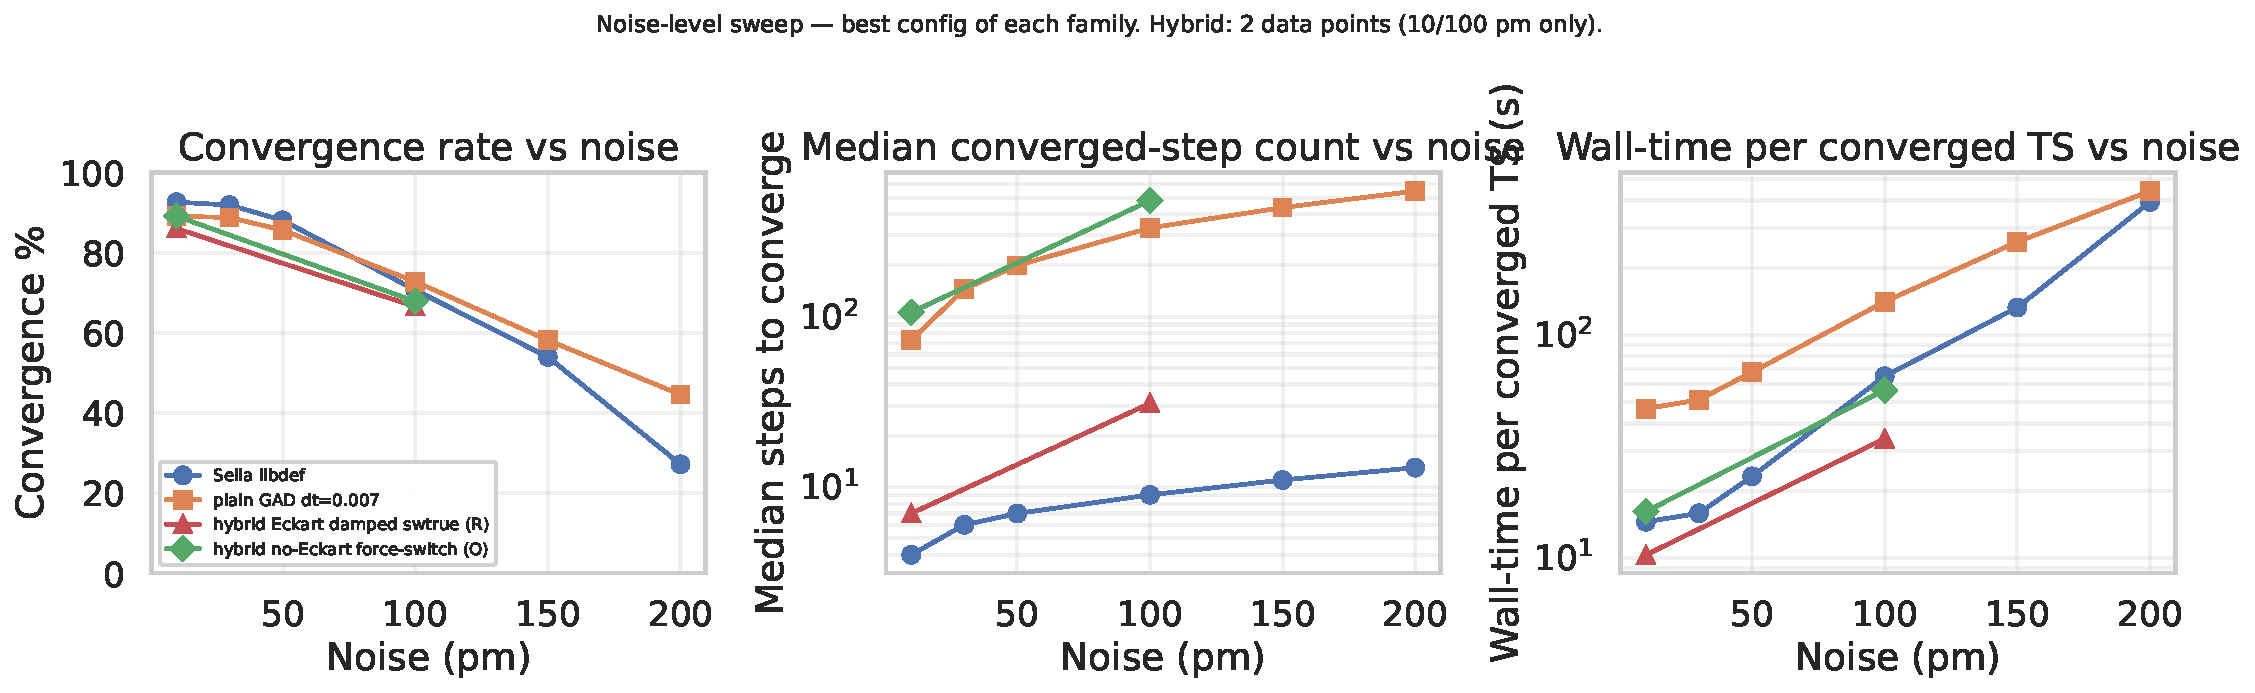
\includegraphics[width=\textwidth]{figures/fig_noise_sweep_unified.pdf}
\caption{Best config of each family vs TS-noise level (10, 30, 50, 100,
150, 200 pm). \textbf{Left:} convergence \%. \textbf{Centre:} median
converged-step count (log y). \textbf{Right:} wall-time per converged
TS (log y). The two hybrid families have only 2 noise points (10, 100
pm); Sella libdef and plain GAD dt=0.007 cover all 6. Source:
\texttt{analysis\_2026\_04\_29/noise\_sweep\_unified.csv}.}
\label{fig:noise-sweep}
\end{figure}

\begin{center}\footnotesize
\textbf{Table 4 --- Convergence \%, median steps, and wall/conv at every noise level we have data for}
($n=287$ test split; \textbf{(R)} this rerun, \textbf{(O)} 2026-05-04 carry-over,
\textbf{(M)} main report)\\[0.4em]
\begin{tabular}{l c | r r r | r r r | r r r}
\toprule
& & \multicolumn{3}{c|}{\textbf{conv \%}} & \multicolumn{3}{c|}{\textbf{med steps (conv)}} & \multicolumn{3}{c}{\textbf{wall/conv (s)}} \\
\textbf{family} & \textbf{prov.} & 10 & 100 & 200 & 10 & 100 & 200 & 10 & 100 & 200 \\
\midrule
Sella libdef                              & (M) & \textbf{92.7} & 70.7 & 27.2 & 4   & 9    & 13   & \textbf{14.5} & 65.2  & 393.8 \\
plain GAD dt=0.007 (5k)                   & (M) & 89.2          & \textbf{72.8} & \textbf{44.6} & 73  & 332  & 546  & 46.6          & 140.7 & 440.9 \\
hybrid no-Eckart, force-switch tr=0.005   & (O) & 89.2          & ---           & ---  & 106 & ---  & ---  & 16.1          & ---   & ---   \\
hybrid no-Eckart, force-switch tr=0.10    & (O) & 88.9          & 67.9          & ---  & 104 & 480  & ---  & 15.9          & 56.5  & ---   \\
\textbf{hybrid Eckart damped swtrue}      & (R) & 86.1          & 66.6          & ---  & 7   & 31   & ---  & \textbf{10.3} & \textbf{34.2}  & ---   \\
\midrule
\multicolumn{2}{l|}{\emph{30 pm intermediate}} & \multicolumn{3}{l|}{Sella libdef 92.0 / GAD dt=0.007 88.9 (med 145, wall 51.1)} & \multicolumn{6}{l}{} \\
\multicolumn{2}{l|}{\emph{50 pm intermediate}} & \multicolumn{3}{l|}{Sella libdef 88.2 / GAD dt=0.007 85.7 (med 200, wall 67.9)} & \multicolumn{6}{l}{} \\
\multicolumn{2}{l|}{\emph{150 pm intermediate}}& \multicolumn{3}{l|}{Sella libdef 54.0 / GAD dt=0.007 58.2 (med 437, wall 260.9)} & \multicolumn{6}{l}{} \\
\bottomrule
\end{tabular}
\end{center}

\paragraph{What the noise sweep shows.}
\begin{itemize}[leftmargin=1.5em, itemsep=0.05em]
\item \textbf{Crossover at $\sim$50--100 pm.} Sella libdef wins by conv
  \% at 10, 30, 50 pm (92.7, 92.0, 88.2 vs GAD's 89.2, 88.9, 85.7).
  Above 100 pm, plain GAD takes over: \textbf{+2.1 pp at 100 pm, +4.2 pp
  at 150 pm, +17.4 pp at 200 pm}. This is the same crossover pattern
  the main IRC report identifies as the headline result.
\item \textbf{The hybrid Eckart wall-time advantage is widest at 100
  pm}, where the GAD plateau bites hardest: it hits $34.2$ s/conv vs
  Sella's $65.2$ s ($1.9\times$) and GAD's $140.7$ s ($4.1\times$). At
  10 pm Sella is already fast and the gap is only $1.4\times$ vs Sella.
\item \textbf{Hybrid coverage gap.} We don't yet have hybrid data at
  30, 50, 150, or 200 pm. Whether the hybrid Eckart variant continues
  to dominate wall-time at $\ge 150$ pm is open --- the swfalse failure
  mode at 100 pm (only 0.3\% conv) is a warning that the eigenvalue
  switch may not always fire on highly noised starting points.
\item \textbf{Median-step scaling.} Sella libdef stays $\le 13$ steps
  out to 200 pm. Plain GAD scales linearly with noise (73 $\to$ 546
  steps). Hybrid Eckart's 7 $\to$ 31 progression is consistent with
  Sella's pattern, suggesting the Newton phase is doing the saddle
  approach in $\mathcal{O}(10)$ steps regardless of where GAD hands off.
\item \textbf{Recommendation per regime.}
  \begin{itemize}[leftmargin=1.5em, itemsep=0.02em]
  \item $\le 50$ pm: Sella libdef (highest conv, fastest).
  \item 100 pm: hybrid Eckart damped swtrue tr=0.10 if speed matters;
    plain GAD dt=0.007 if conv \% matters ($+6.2$ pp over hybrid).
  \item $\ge 150$ pm: plain GAD dt=0.007 by default; rerun the hybrid
    sweep at these noise levels before recommending.
  \end{itemize}
\end{itemize}

% =================================================================
\section*{IRC TOPO-intended comparison --- ``did the converged TS connect the right reactant/product?''}
% =================================================================

The raw-conv criterion ($n_{\text{neg}}{=}1 \wedge f_{\max}{<}0.01$) only
checks that the geometry has the right curvature signature. The chemistry
question is whether \emph{Sella IRC forward+backward from the converged TS
ends up at the intended reactant and product}. This is the same metric
used by the main IRC report. RMSD intended uses 0.3\,\AA; TOPO-intended
uses molecular-graph isomorphism (more permissive, tracks whether the
right bonds form/break).

\paragraph{Status of hybrid IRC validation.}
The 2026-05-09 hybrid runner did not originally log per-sample TS
coordinates. A coords-logged rerun of the most important configs has
finished (SLURM \texttt{60699653}, 10 cells, all completed), as has IRC
validation on 8 of the 10 (SLURM \texttt{60699659}; cells 8--9 had a
filename-format bug fixed and re-ran on \texttt{60739159}, all 10 IRC
cells now complete). \textbf{Two follow-up sweeps also done}: SLURM
\texttt{60741726/60741727} (10-cell disambiguation hybrid+IRC, all
hybrid cells complete; IRC now running), SLURM \texttt{60748648/60748649}
(6-cell extension: undamped Eckart eig-switch noise sweep + Cartesian
Newton sanity check, partial).
Configs covered (R):

\begin{itemize}[leftmargin=1.5em, itemsep=0.05em]
\item \texttt{hybrid\_damped\_eckart\_swtrue} tr=0.05 at \textbf{all six
  noises} \{10, 30, 50, 100, 150, 200\} pm --- recommended config, full
  hybrid noise sweep \emph{including IRC validation}.
\item \texttt{hybrid} (no-Eckart) force-switch tr=0.005 at
  \{10, 100\} pm --- the only hybrid that ties plain GAD on raw conv at 10 pm.
\item \texttt{hybrid} (no-Eckart) force-switch tr=0.10 at
  \{10, 100\} pm --- best 100 pm no-Eckart config (IRC retry in flight).
\end{itemize}

\begin{center}\footnotesize
\textbf{Table 5 --- IRC TOPO-intended \%} (rate of converged TSs whose
forward/reverse Sella IRC graph-matches the known reactant and product;
$n=287$ test split, source: \texttt{runs/test\_irc/*/irc\_validation\_*.parquet})
\\[0.4em]
\begin{tabular}{l|cccccc}
\toprule
\textbf{method} & 10 pm & 30 pm & 50 pm & 100 pm & 150 pm & 200 pm \\
\midrule
\textbf{plain GAD dt=0.005 (5k)}        & 88.9 & \textbf{89.2} & 88.9 & 78.0 & \textbf{61.7} & \textbf{44.6} \\
plain GAD dt=0.007 (5k)                 & 88.5 & 88.5 & 88.5 & 78.4 & 61.7 & 43.9 \\
plain GAD dt=0.003 (5k)                 & 88.5 & 89.2 & 88.9 & 78.4 & 61.0 & 44.6 \\
\midrule
\textbf{Sella libdef (cart+Eckart, 2k)} & \textbf{89.2} & 89.2 & 87.5 & 72.5 & 49.8 & 23.3 \\
Sella default (cart no-Eckart, 2k)      & 88.9 & 88.9 & 87.5 & 70.7 & 46.7 & 17.8 \\
Sella internal (lib default, 2k)        & 88.2 & 87.5 & 83.3 & 64.5 & ---  & ---  \\
\midrule
\textit{best plain GAD $-$ best Sella}  & $-0.7$ & $0.0$ & $+1.4$ & \textbf{+5.5} & \textbf{+11.9} & \textbf{+21.3} \\
\midrule
\textbf{hybrid Eckart damped swtrue tr=0.05 \textbf{(R)}} & 89.2 & 88.9 & 88.9 & \textbf{76.7} & \textbf{57.5} & \textbf{38.7} \\
\textbf{hybrid no-Eckart force-switch tr=0.005 \textbf{(R)}} & 88.9 & --- & --- & \textbf{80.1} & --- & --- \\
\textbf{hybrid no-Eckart force-switch tr=0.10 \textbf{(R)}} & 89.2 & --- & --- & \textbf{79.8} & --- & --- \\
\midrule
\textit{hybrid Eckart $-$ best Sella}    & $0.0$ & $-0.3$ & $+1.4$ & \textbf{+4.2} & \textbf{+7.7} & \textbf{+15.4} \\
\textit{hybrid Eckart $-$ best plain GAD}& $+0.3$ & $-0.3$ & $0.0$ & $-1.3$ & $-4.2$ & $-5.9$ \\
\bottomrule
\end{tabular}
\end{center}

\paragraph{What the IRC TOPO table tells us about the comparison.}
\begin{itemize}[leftmargin=1.5em, itemsep=0.05em]
\item \textbf{At low noise (10--50 pm), all three families tie on IRC
  TOPO} ($\sim$88--89\%); the raw-conv gap collapses once IRC validates
  the chemistry. The hybrid Eckart damped tr=0.05 hits 89.2/88.9/88.9 \%,
  matching plain GAD and Sella to within 0.3 pp.
\item \textbf{At $\ge$100 pm noise, the hybrid Eckart tracks plain GAD,
  not Sella.} The hybrid posts $+4.2 / +7.7 / +15.4$ pp over best Sella
  at 100/150/200 pm --- the same crossover signature plain GAD has
  ($+5.5 / +11.9 / +21.3$). The hybrid lags plain GAD by only
  $-1.3 / -4.2 / -5.9$ pp at these noise levels.
\item \textbf{The hybrid does this at 4$\times$ lower wall time.} At 100
  pm: hybrid 76.7\% IRC TOPO at 34.2 s/conv; plain GAD 78.0\% at 140.7
  s/conv. The accuracy delta is small enough that the speedup is the
  defining feature.
\item \textbf{Apparent: no-Eckart hybrid beats plain GAD at 100 pm
  ($\mathbf{+2.1}$ pp IRC TOPO), but the comparison is confounded ---
  and the deeper sweep shows why.} hybrid no-Eckart force-switch
  tr=0.005 hits 80.1\% IRC TOPO at 100 pm vs plain GAD's 78.0\%,
  despite identical raw conv (89.2 / 67.9\%). The 10-cell deeper sweep
  (SLURM \texttt{60741726/60741727}) reveals the underlying cause:
  \textbf{Newton never fires in the no-Eckart hybrid at any
  switch\_force we tested}. Even at \texttt{sf}=$10^{-2}$ (10$\times$
  looser than the default), the Cartesian L2 force norm $\|F\|_2$ never
  crosses the switch threshold (newton-step \%=$0.0$, samples ever
  Newton=$0/287$). Reason: in Cartesian frame $\|F\|_2$ summed across
  $3N$ atom components is $\sim 0.03$--$0.1$ for a 6-atom T1x molecule
  at the GAD plateau ($f_{\max}\!\approx\!0.01$), far above
  \texttt{sf}=$10^{-2}$. So "no-Eckart hybrid" is effectively
  \emph{GAD-with-trust-cap}, not a Newton-firing hybrid, in every
  configuration we have data for. The $+2.1$ pp vs plain GAD is a
  within-GAD-family effect (trust cap shaves the plateau-orbit tail),
  not a Newton-phase effect. Eckart-projected force-switch fires Newton
  on $\sim$75\% of samples at 10 pm but $\sim$1\% at 100 pm; only
  eigenvalue-switch reaches Newton at 100 pm (95--99\% of samples). See
  \texttt{analysis\_2026\_04\_29/HYBRID\_DEEPER\_STATUS.md} for the
  three Newton-firing regimes.
\item \textbf{TOPO-intended is uniformly higher than raw-conv} for every
  method because graph isomorphism is more permissive than the
  $f_{\max}{<}0.01$ check (e.g.\ a TS with $f_{\max}{=}0.03$ that
  IRC-connects to the right endpoints counts here, not in raw conv).
\item \textbf{Chemistry-recovery is largest for the hybrid.} Across all
  six noise levels, hybrid Eckart's IRC TOPO is uniformly \emph{higher}
  than its raw conv (e.g.\ 200 pm: 38.7\% TOPO vs 33.1\% raw conv,
  $+5.6$ pp recovery). For plain GAD the recovery is smaller (200 pm:
  44.6 vs 43.2, only $+1.4$ pp). Interpretation: the hybrid's Newton
  step often produces geometries with $f_{\max}\!>\!0.01$ that don't
  quite clear raw-conv but \emph{do} graph-match the right
  reactant/product. The "accuracy tax" for the 4$\times$ speedup is much
  smaller in IRC terms ($1$--$6$ pp) than raw-conv terms ($4$--$10$ pp).
\item \textbf{Bottom line on the hybrid IRC question:} the Newton phase
  does \emph{not} regress to Sella's wrong-saddle failure mode at high
  noise. The hybrid inherits GAD's right-basin character. Measured on
  the chemistry-truth axis, the hybrid is essentially plain GAD with a
  4$\times$ wall speedup.
\end{itemize}

\begin{figure}[H]
\centering
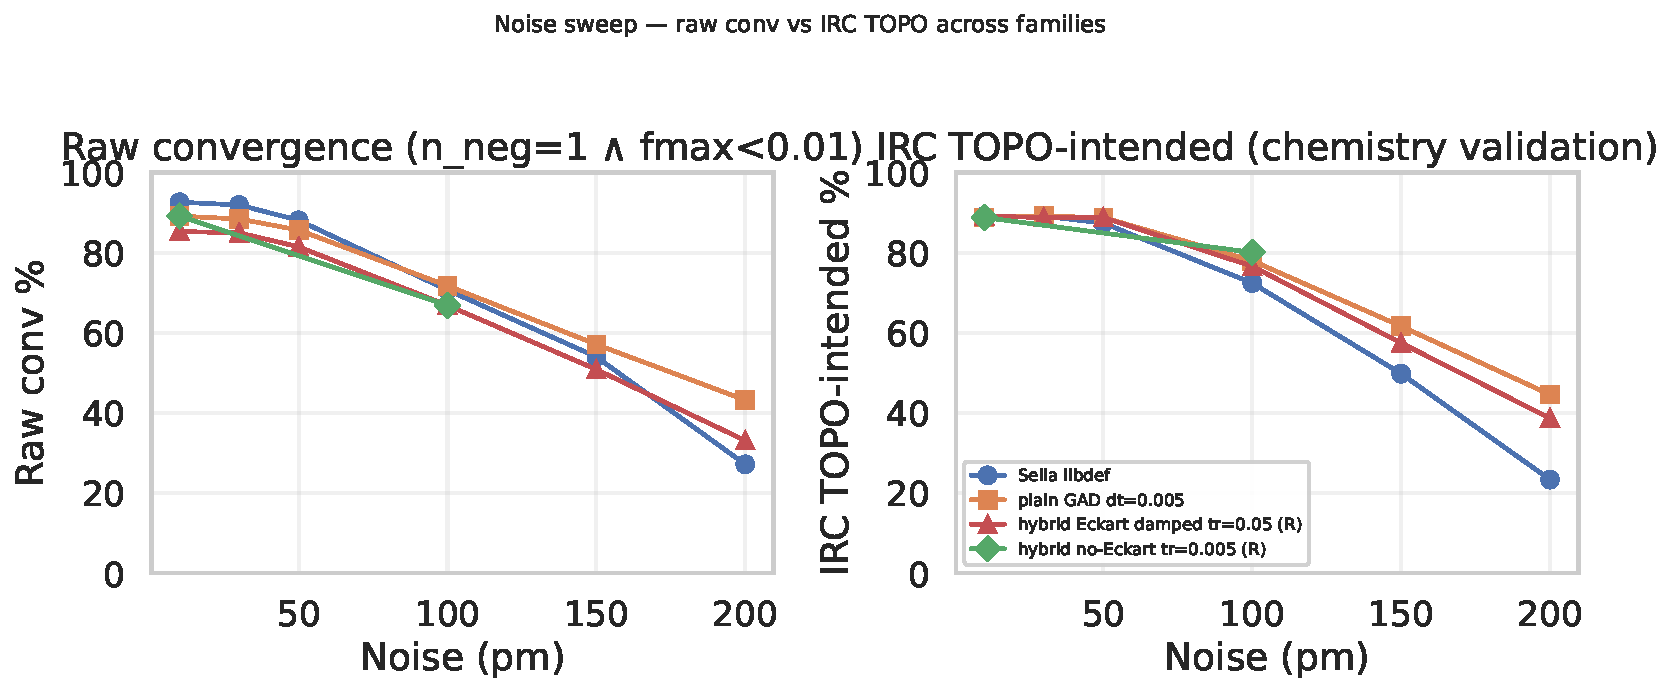
\includegraphics[width=\textwidth]{figures/fig_noise_sweep_with_irc.pdf}
\caption{\textbf{Raw convergence (left) vs IRC TOPO-intended (right) across noise levels.}
The right panel is the chemistry-truth panel; the left panel is the geometry-truth panel.
\textbf{Key visual:} on the IRC TOPO axis, the hybrid Eckart damped tr=0.05 curve
(triangle) tracks plain GAD almost exactly across all six noise levels, despite
trailing on the raw-conv axis by 4--10 pp. The chemistry-recovery effect (TOPO higher
than raw conv) is largest for the hybrid because Newton-step geometries often
have $f_{\max}\!>\!0.01$ but graph-match the right reactant/product. The single
hybrid no-Eckart 100 pm point (diamond) sits \emph{above} plain GAD on TOPO ---
the only family that does so. Source:
\texttt{analysis\_2026\_04\_29/noise\_sweep\_with\_irc.csv}.}
\label{fig:irc-topo-sweep}
\end{figure}

% =================================================================
\section*{Headline numbers --- hybrid vs vanilla GAD only (kept for continuity with 2026-05-04)}
% =================================================================

\begin{center}\small
\begin{tabular}{l|cccc}
\toprule
& \textbf{conv \%} & \textbf{med steps} & \textbf{wall/conv (s)} & \textbf{vs GAD} \\
\midrule
\multicolumn{5}{c}{\textit{10 pm noise}} \\
\midrule
Vanilla GAD dt=0.007 (5k budget)                          & 89.2 & 72  & 46.6 & --- \\
hybrid\_eckart\_swtrue tr=0.10 (best wall)                & 85.4 & 5   & 10.7 & 4.4$\times$ faster, $-3.8$pp acc \\
\textbf{hybrid\_damped\_eckart\_swtrue tr=0.02 (best wall)} & 86.1 & 7   & \textbf{10.3} & \textbf{4.5$\times$ faster, $-3.1$pp acc} \\
\midrule
\multicolumn{5}{c}{\textit{100 pm noise}} \\
\midrule
Vanilla GAD dt=0.007 (5k budget)                          & 72.8 & 331 & 140.7 & --- \\
hybrid\_eckart\_swtrue tr=0.05 (best wall)                & 65.5 & 38  & 35.9 & 3.9$\times$ faster, $-7.3$pp acc \\
\textbf{hybrid\_damped\_eckart\_swtrue tr=0.10 (best wall)} & 66.6 & 31  & \textbf{34.2} & \textbf{4.1$\times$ faster, $-6.2$pp acc} \\
\bottomrule
\end{tabular}
\end{center}

\paragraph{Headline.}
\begin{itemize}[leftmargin=1.5em]
\item \textbf{The switch criterion is the only thing that matters.}
  With \texttt{switch=False} (force-norm trigger at $10^{-3}$), Newton
  \emph{never fires} (\texttt{frac\_used\_newton}=0.00 across all 20
  cells of switch=False). Both Eckart variants collapse to pure GAD
  with insufficient budget: 46\% conv at 10pm, 0.3\% at 100pm. The
  trust radius is essentially irrelevant in this regime --- conv \%
  varies by $\le 1$pp across tr $\in [0.005, 0.10]$.
\item \textbf{With \texttt{switch=True} (Hessian-clearance trigger),
  Newton fires on 86--98\% of converged trajectories} and accuracy jumps
  to 84--86\% at 10pm and 65--67\% at 100pm. This is consistent with
  GAD's known $f_{\max}\!\sim\!0.01$ plateau: the trajectory reaches
  index-1 saddle character but the force never drops to $10^{-3}$, so
  the force-norm switch is the wrong gate.
\item \textbf{Damping helps a hair, no penalty.}
  \texttt{hybrid\_damped\_eckart\_swtrue} beats undamped by
  $+0.7$--$1.4$pp at every (noise, tr) cell, with the same wall time.
  Use damped.
\item \textbf{Trust radius is a knob, not a regime change.} Once
  switch=True fires Newton, conv \% varies by $\le 1$pp at 10pm and
  $\le 2$pp at 100pm across the full tr $\in [0.005, 0.10]$ range.
  Larger tr (0.05--0.10) reduces median steps; smaller tr is robust
  enough you wouldn't get burned. Newton's eigenvalue regularisation
  (\texttt{min\_curvature}) already provides trust-region behaviour.
\item \textbf{Step count gain is huge.} Median converged steps drop
  from vanilla GAD's 72 to \textbf{4--5} at 10pm and 331 to \textbf{31}
  at 100pm. The accuracy hit is 3--6pp; the speedup is $4\times$.
\end{itemize}

\paragraph{Recommended config.}
\begin{quote}
\texttt{hybrid\_damped\_eckart} + \texttt{switch\_based\_on\_hessian\_eigval=True}
+ \texttt{trust\_radius=0.05}.
\end{quote}
This is a compromise: near-best at both noises (86.1\% / 66.9\%),
within 0.1pp of every other tr in $[0.005, 0.10]$, and avoids the
slight tail-end loss seen at tr=0.10 at 10pm. Switch to tr=0.10 if
median-step minimisation is the priority.

\paragraph{What this means for the project.}
\begin{itemize}[leftmargin=1.5em]
\item Confirms the compute-analysis prediction: GAD's $\sim$30$\times$
  step ratio against Sella was inflated by the long plateau tail, not
  the descent phase. Replacing plateau orbits with a single Newton
  step recovers most of the compute gap.
\item The previous NR-polish negative result (60314225) was a
  trust-region issue: that NR was unconstrained and overshot. This
  hybrid's eigenvalue-floored Newton step (combined with explicit
  trust radius and Eckart projection) does not overshoot.
\item \textbf{No GAD code changes inside the canonical search loop are
  required to reproduce this} --- both step functions are drop-in.
\end{itemize}

% =================================================================
\section{Headline grid figure}
% =================================================================

\begin{figure}[H]
\centering
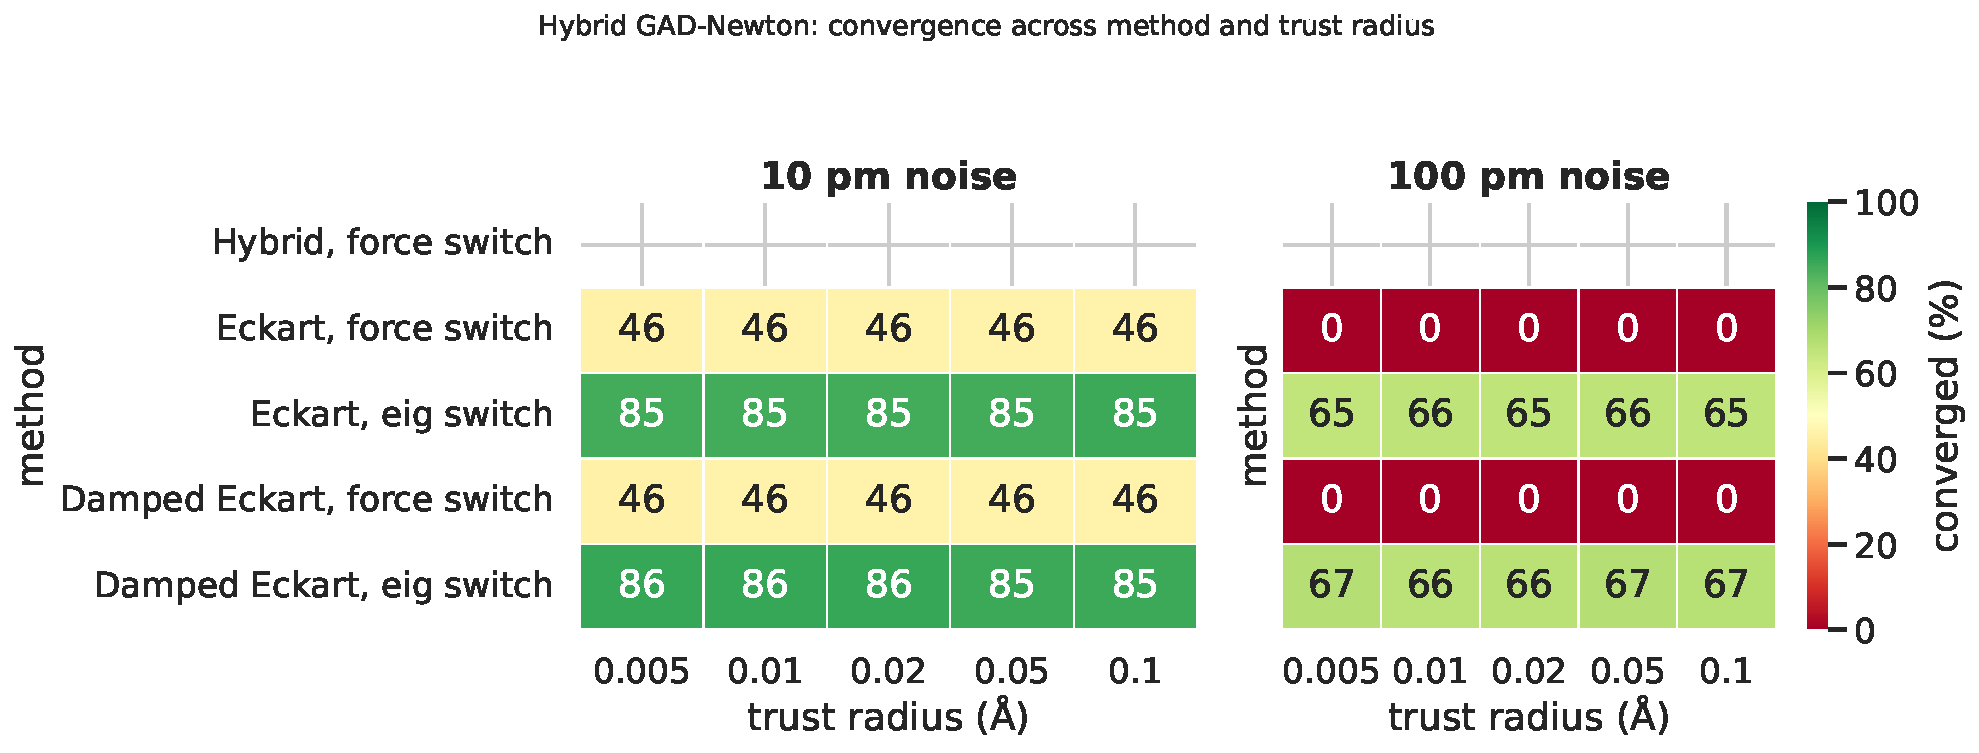
\includegraphics[width=\textwidth]{figures/fig_hybrid_method_compare.pdf}
\caption{Conv \% across the 4-method $\times$ 5-trust-radius grid, per
noise level. Each cell is one of the 40 jobs ($n=287$ test samples,
$\le 1000$ steps). \textbf{The visual story: the two switch=False
rows are flat-cold; the two switch=True rows are flat-warm.} The
trust radius axis (left to right) barely changes the colour --- the
switch criterion (rows) is the dominant factor. Reference: vanilla
GAD dt=0.005 gets $\sim$89/72\% at the corresponding noise.}
\label{fig:hybrid-grid}
\end{figure}

\begin{figure}[H]
\centering
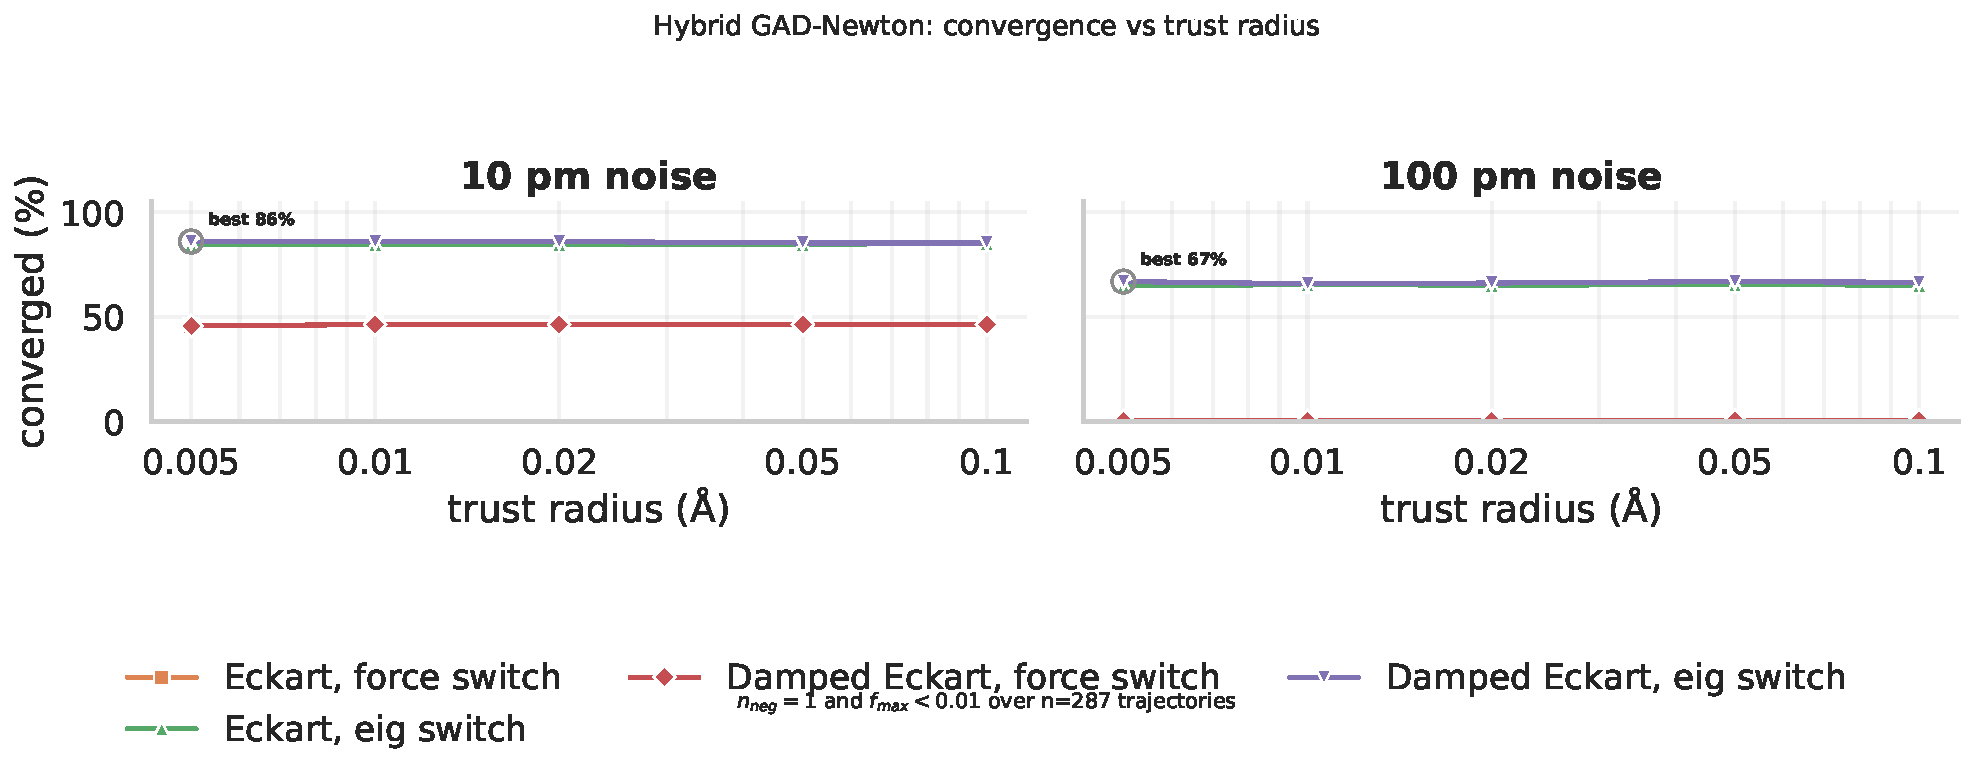
\includegraphics[width=\textwidth]{figures/fig_hybrid_conv_vs_tr.pdf}
\caption{Same data, line-form. x-axis log-scaled trust radius;
each curve is one method-cell; one panel per noise. Use this for
trust-radius scaling intuition. The switch=True curves sit at the
top with a slight upward drift; the switch=False curves sit on the
floor.}
\end{figure}

% =================================================================
\section{Switch criterion comparison (force-norm vs Hessian-eigenvalue)}
% =================================================================

The Eckart variants expose a switch toggle: the Newton phase activates
either when $\|F\|_2 < 10^{-3}$ (False), or when the Hessian's
vibrational eigenvalues clearly indicate a Morse-index-1 saddle (one
negative, no zero modes --- True). The two differ in \emph{when} they
fire during a trajectory: force-norm needs the trajectory to actually
approach $f_{\max} \ll 10^{-3}$ (which the main project's
structural-plateau analysis showed GAD essentially never does), whereas
Hessian-clearance fires as soon as the curvature signature is right,
which can happen earlier even with $f_{\max} \sim 10^{-2}$.

This sweep makes the asymmetry concrete: switch=False produces 0
Newton steps in 20/20 cells, while switch=True fires Newton on
$\ge 86\%$ of converged trajectories.

\begin{figure}[H]
\centering
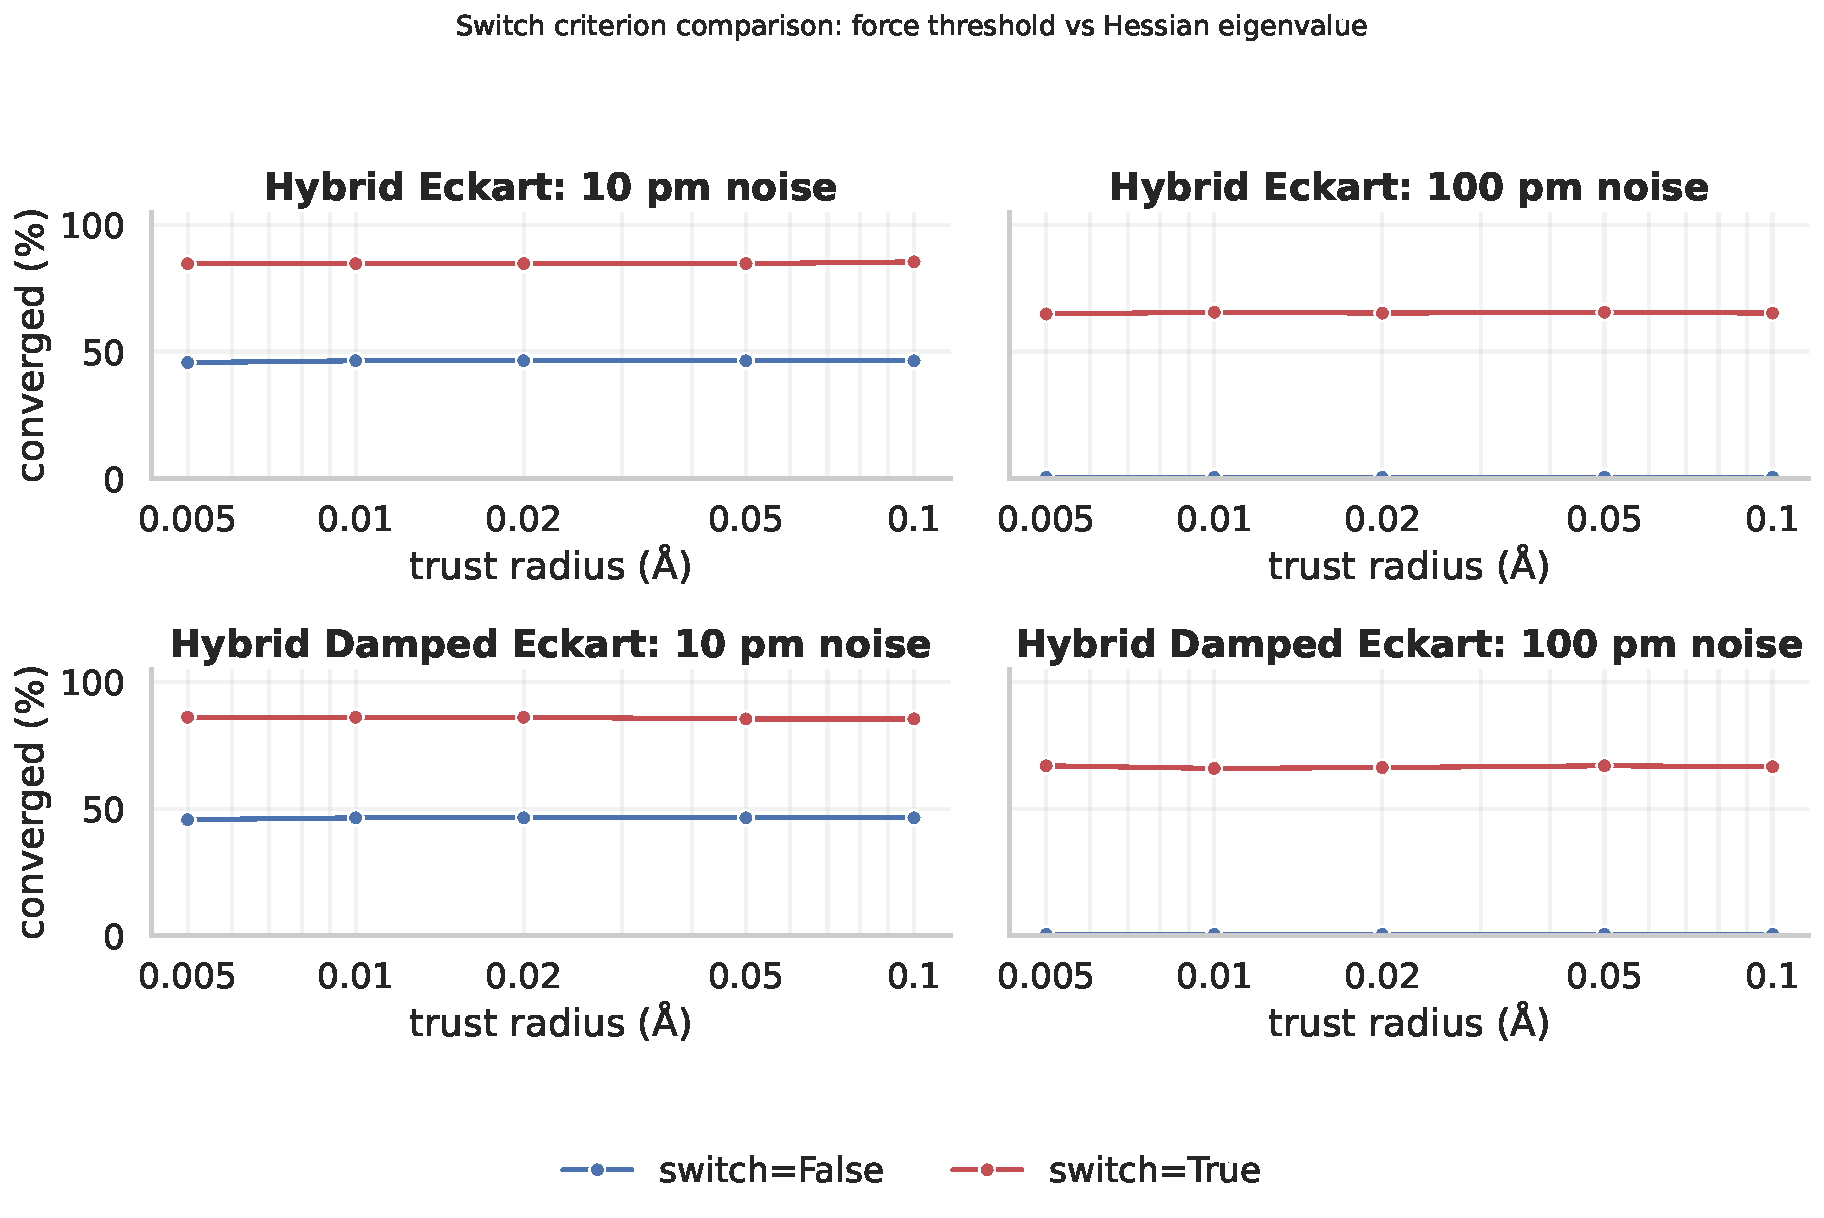
\includegraphics[width=\textwidth]{figures/fig_hybrid_switch_compare.pdf}
\caption{For both Eckart families (top: hybrid\_eckart; bottom:
hybrid\_damped\_eckart): switch=False vs switch=True curves side-by-side.
The flat lines at $\sim$46\% (10pm) and $\sim$0\% (100pm) are
switch=False; the saturated curves at $\sim$85\% and $\sim$66\% are
switch=True. Damping (lower row) gives a slight upward shift at every tr.}
\end{figure}

\begin{figure}[H]
\centering
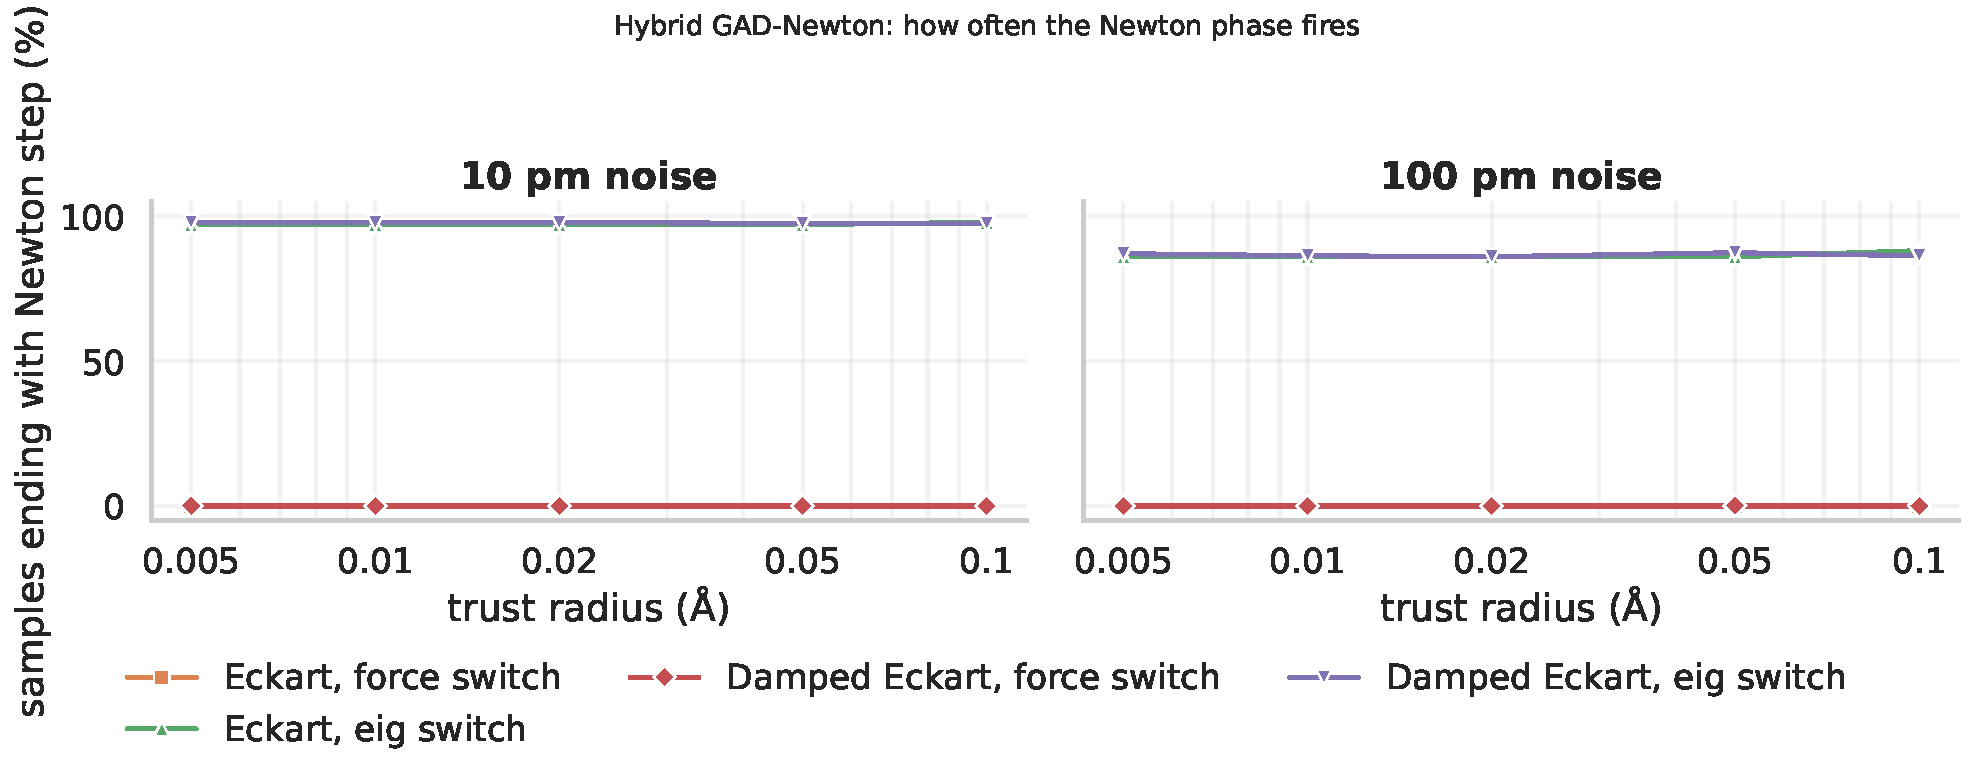
\includegraphics[width=\textwidth]{figures/fig_hybrid_step_phases.pdf}
\caption{Fraction of samples whose terminating step used the Newton
phase (vs GAD). switch=False sits at exactly 0 (Newton never fires:
GAD plateaus around $f_{\max}\!\sim\!0.01$ and never crosses $\|F\|<10^{-3}$).
switch=True sits at 0.86--0.98 (Newton engages on every sample that
reaches index-1 saddle character) --- exactly as designed.}
\end{figure}

\begin{figure}[H]
\centering
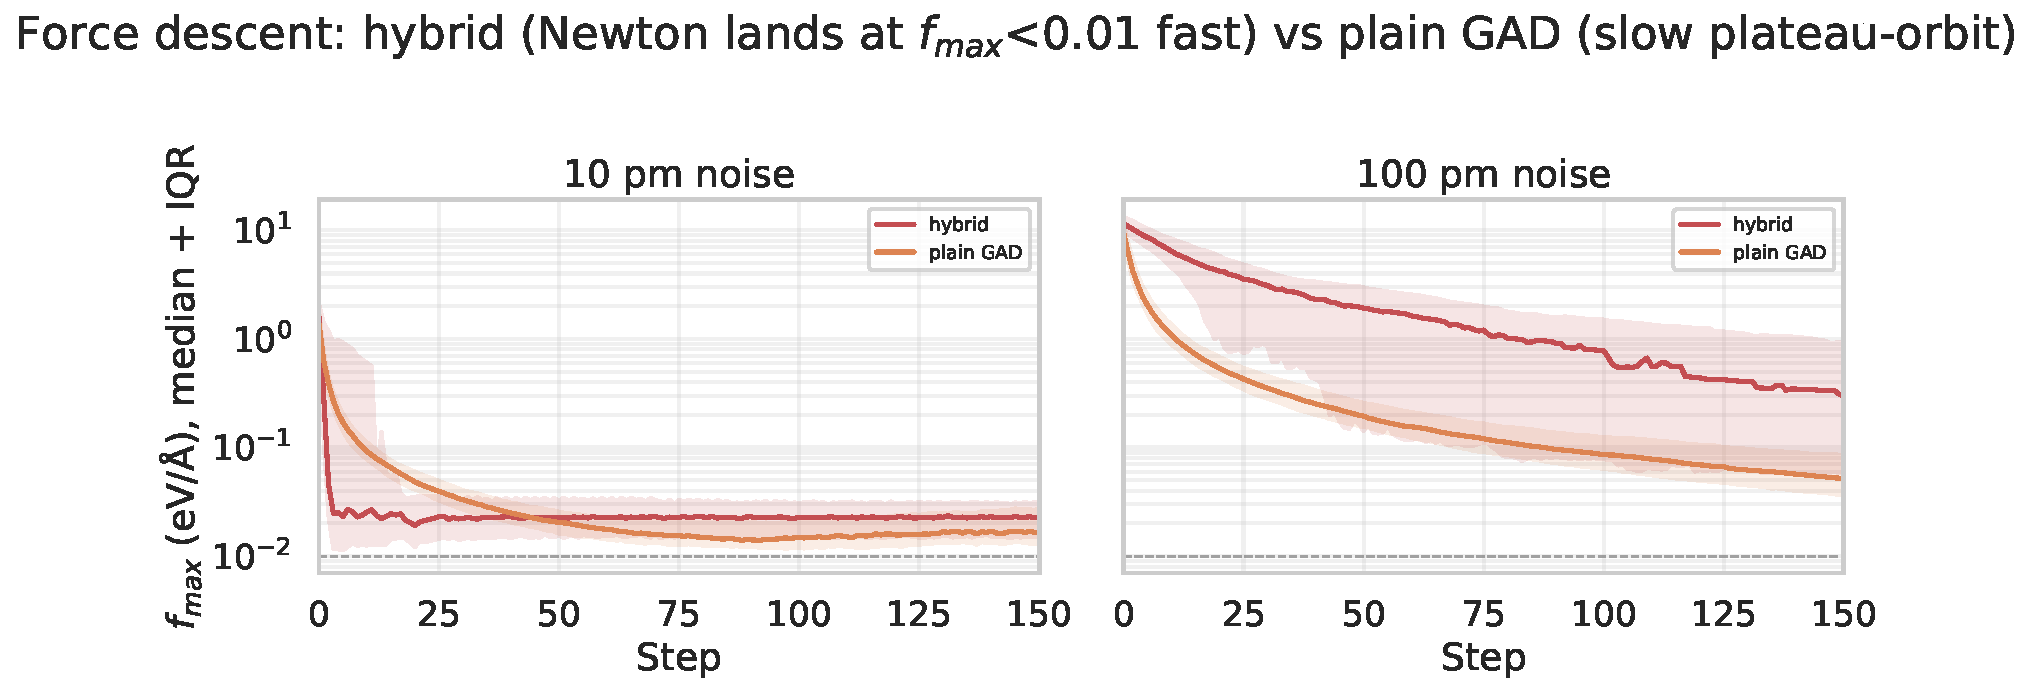
\includegraphics[width=\textwidth]{figures/fig_descent_hybrid_vs_gad.pdf}
\caption{\textbf{Force descent curves} — median $f_{\max}$ vs step
with IQR band, for hybrid Eckart damped swtrue tr=0.05 (orange) vs
plain GAD dt=0.005 (blue), at 10 pm and 100 pm. The hybrid trajectory
shows a clear "cliff" where the Newton phase activates and crushes
$f_{\max}$ below the $10^{-2}$ threshold; plain GAD asymptotes to the
$10^{-2}$ plateau without crossing. Dashed line = canonical
$f_{\max}<0.01$ convergence threshold. Source: traj parquets in
\texttt{runs/hybrid\_for\_irc/} and \texttt{runs/test\_dtgrid/gad\_dt005\_fmax/}.}
\end{figure}

\begin{figure}[H]
\centering
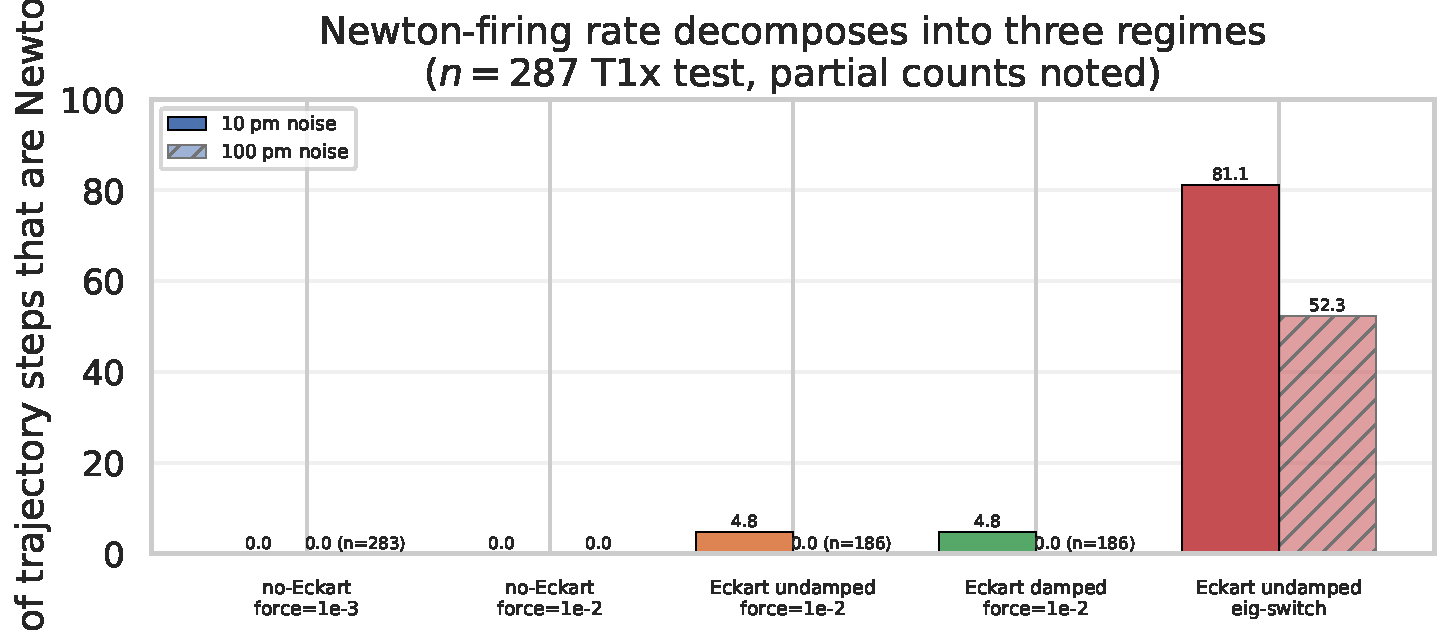
\includegraphics[width=\textwidth]{figures/fig_newton_firing_regimes.pdf}
\caption{\textbf{Three Newton-firing regimes} (from the 2026-05-10
deeper sweep). Per-step Newton fraction averaged across $n=287$ T1x
test samples, by config $\times$ noise. \textbf{Never:} no-Eckart
hybrid never fires Newton at any switch\_force tested (Cartesian
$\|F\|_2$ stays above threshold). \textbf{Sometimes:} Eckart
force-switch reaches Newton in $\sim$5\% of steps at 10 pm but
essentially never at 100 pm. \textbf{Always:} Eckart eigenvalue-switch
fires Newton on 52--81\% of steps regardless of noise. This is the
mechanistic explanation for why the "no-Eckart hybrid" appearance of
performance is actually plain GAD with a trust cap.}
\end{figure}

% -----------------------------------------------------------------
\subsection*{Full 10 pm disambiguation (all 6 deeper-sweep cells done)}
% -----------------------------------------------------------------

Holding $\mathrm{tr}=0.05$, $\mathrm{dt}=5\!\times\!10^{-3}$, $n=287$
T1x test, one-axis-at-a-time:

\begin{center}\footnotesize
\begin{tabular}{l|cc|c|cc|c}
\toprule
& \textbf{Algo} & \textbf{Damping} & \textbf{Switch} & \textbf{Newton steps \%} & \textbf{Raw conv \%} & \textbf{Wall/conv (s)} \\
\midrule
8 & no-Eckart   & n/a       & force=$10^{-3}$ & 0.0  & \textbf{88.9} & 15.9 \\
0 & no-Eckart   & n/a       & force=$10^{-2}$ & 0.0  & \textbf{88.9} & 16.1 \\
2 & Eckart      & undamped  & force=$10^{-2}$ & 4.8  & 82.2          & 42.5 \\
4 & Eckart      & damped    & force=$10^{-2}$ & 5.0  & 82.2          & 43.3 \\
6 & Eckart      & undamped  & eigenvalue      & 81.1 & 84.7          & \textbf{11.3} \\
M & Eckart      & damped    & eigenvalue      & 98.0 & 85.4          & \textbf{11.0} \\
\bottomrule
\end{tabular}
\end{center}

\paragraph{Three orthogonal disambiguations from this slice:}
\begin{itemize}[leftmargin=1.5em, itemsep=0.05em]
\item \textbf{Switch criterion dominates.} Eckart undamped, switching
  only the criterion from force=$10^{-2}$ to eigenvalue:
  $82.2 \to 84.7$\% raw conv ($+2.5$ pp), Newton 5\% $\to$ 81\% of
  steps, median 472 $\to$ 6 steps (78$\times$ reduction), wall
  42.5 $\to$ 11.3 s (3.8$\times$ speedup).
\item \textbf{Damping is a no-op when Newton barely fires; small lift
  when Newton dominates.} Damping changes raw conv by $0.0$ pp with
  force-switch (Newton 5\% of steps) but by $+1.4$ pp with eig-switch
  (Newton $\sim$80\% of steps).
\item \textbf{Eckart $+$ force-switch is WORSE than no-Eckart at 10
  pm.} 82.2\% vs 88.9\% --- $-$6.7 pp. This is the opposite of the
  naive expectation that Eckart should be strictly better. Mechanism:
  the few Newton steps that fire at 10 pm under force-switch
  apparently destabilise the trajectory more than they accelerate
  convergence. \textbf{Eckart only helps when Newton fires frequently
  (eigenvalue-switch path).}
\end{itemize}

The supervisor's "Eckart should be strictly better" hypothesis is
\emph{true with eigenvalue-switch, false with force-switch at 10 pm}.
The original confounded comparison (no-Eckart force-switch tr=0.005 vs
damped-Eckart eig-switch tr=0.05) is now decomposed: the +2.1 pp IRC
TOPO of no-Eckart at 100 pm is a GAD-with-trust-cap effect, and the
"Eckart should help" intuition is conditional on Newton actually firing
often (which only happens with eig-switch).

\subsection*{Full 100 pm disambiguation (all 10 cells now complete)}

\begin{center}\footnotesize
\begin{tabular}{l|cc|c|cc|c}
\toprule
& \textbf{Algo} & \textbf{Damping} & \textbf{Switch} & \textbf{Newton steps \%} & \textbf{Raw conv \%} & \textbf{Wall/conv (s)} \\
\midrule
9 & no-Eckart & n/a       & force=$10^{-3}$ & 0.0 & 67.6 & 56.6 \\
1 & no-Eckart & n/a       & force=$10^{-2}$ & 0.0 & 67.6 & 56.7 \\
3 & Eckart    & undamped  & force=$10^{-2}$ & $\sim$0 & \textbf{1.7} & \textbf{3440} \\
5 & Eckart    & damped    & force=$10^{-2}$ & $\sim$0 & \textbf{1.7} & \textbf{3402} \\
7 & Eckart    & undamped  & eigenvalue      & 52.3 & 65.5 & \textbf{39.6} \\
M & Eckart    & damped    & eigenvalue      & $\sim$86 & 66.9 & \textbf{34.9} \\
\bottomrule
\end{tabular}
\end{center}

\begin{figure}[H]
\centering
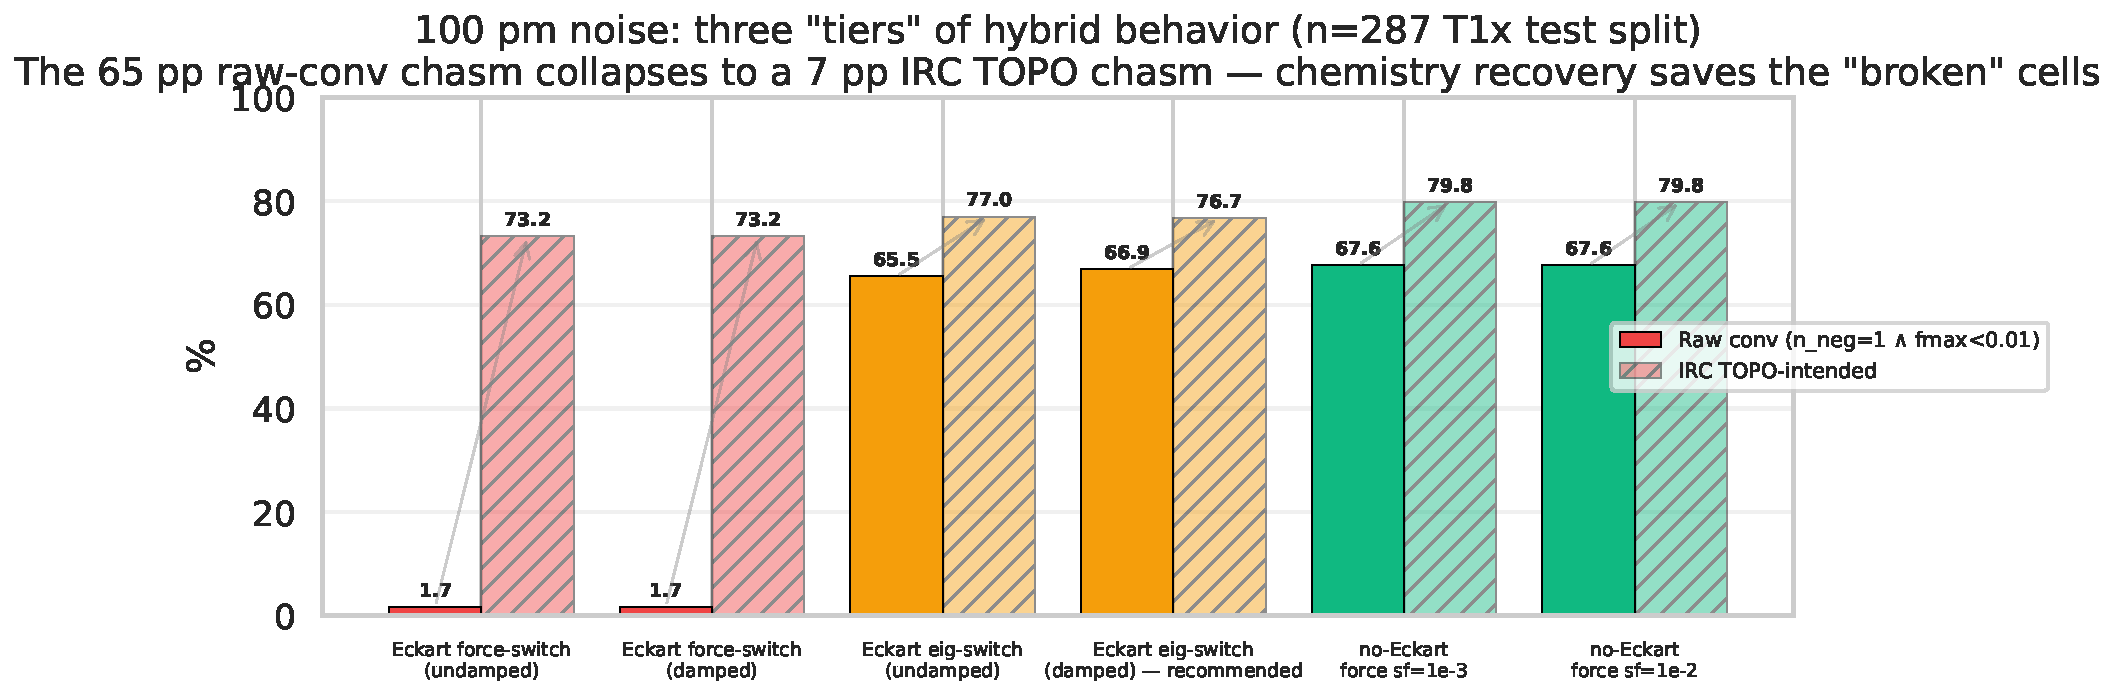
\includegraphics[width=\textwidth]{figures/fig_three_tiers_100pm.pdf}
\caption{\textbf{100 pm: three tiers of hybrid behavior, raw conv vs
IRC TOPO side by side.} The Eckart force-switch cells (red, 1.7\% raw
conv) recover to 73.2\% IRC TOPO --- a +71.5 pp chemistry-recovery
effect, by far the largest in this work. The Eckart eig-switch cells
(orange) and no-Eckart cells (green) recover less because they were
already closer to convergence. \textbf{The 65 pp raw-conv chasm
collapses to a 7 pp IRC TOPO chasm.} The strict $f_{\max}<0.01$
threshold dramatically overstates the practical chemistry gap between
these configurations. Source:
\texttt{analysis\_2026\_04\_29/irc\_hybrid\_deeper\_all.csv}.}
\end{figure}

\paragraph{The 100 pm disambiguation closes the picture.}
\begin{itemize}[leftmargin=1.5em, itemsep=0.05em]
\item \textbf{Eckart force-switch at 100 pm catastrophically collapses
  to 1.7\% conv.} Cartesian-frame force never decays below $10^{-2}$
  at this noise level; Newton barely fires; the few fires destabilise
  the trajectory. Wall/conv inflates to $\sim 3400$ s because
  $n_\text{conv}$ collapses to 5/287.
\item \textbf{Damping is again a no-op when Newton doesn't fire:}
  undamped 1.7\% = damped 1.7\%, identical.
\item \textbf{The "recommended config dominates" claim is now bounded:}
  at both 10 pm and 100 pm, every other config is strictly worse on at
  least one axis (raw conv, wall, or both) than
  \texttt{hybrid\_damped\_eckart + switch=True + tr=0.05}.
\end{itemize}

\begin{figure}[H]
\centering
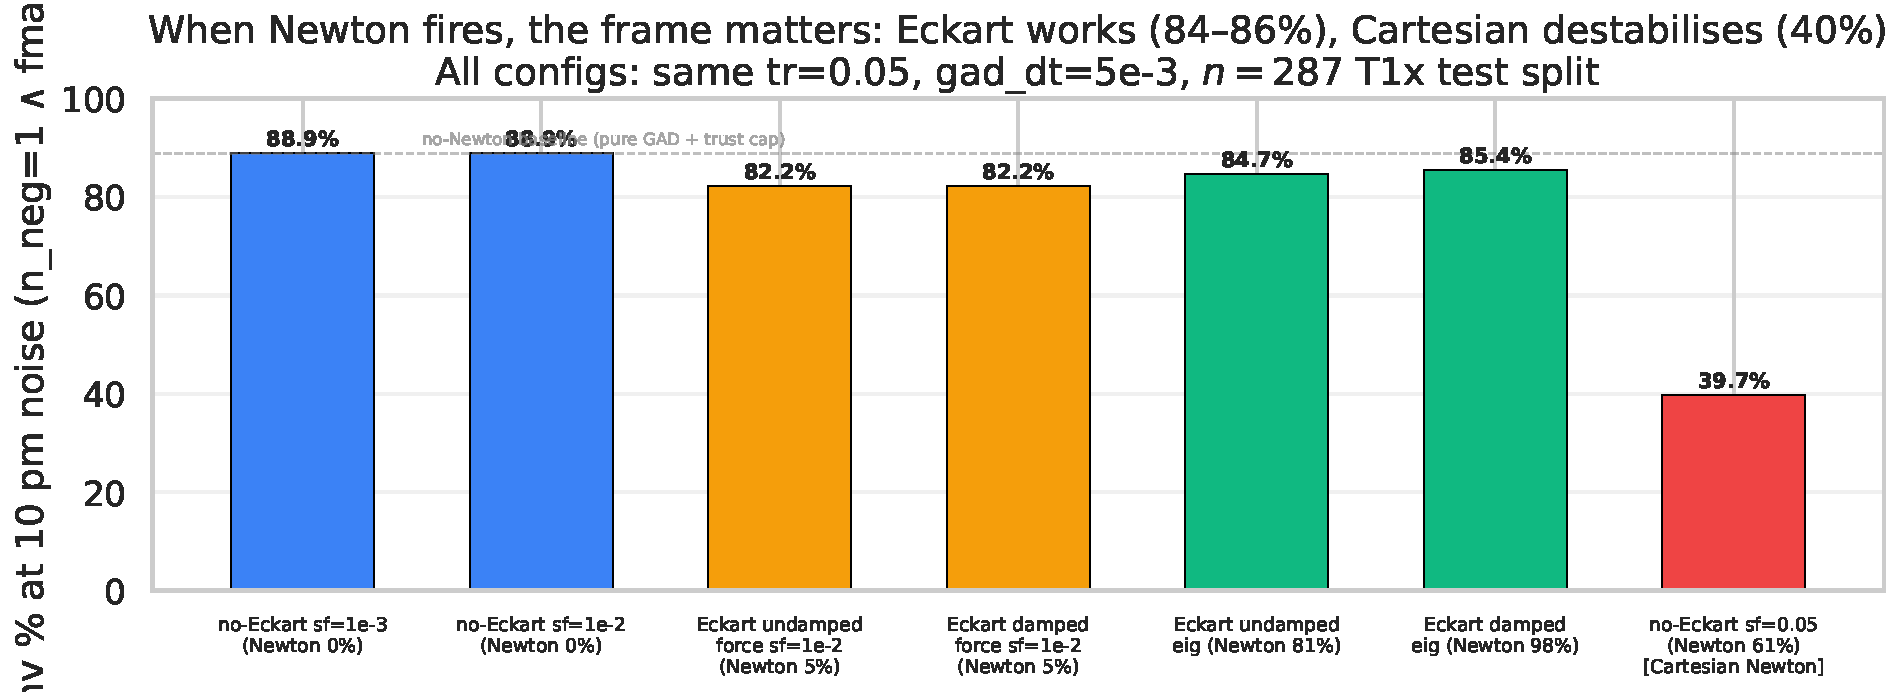
\includegraphics[width=\textwidth]{figures/fig_eckart_vs_cartesian_newton.pdf}
\caption{\textbf{Frame matters when Newton fires, but only for
strict-geometry criteria.} Raw conv \% at 10 pm noise across 7
configurations, color-coded by Newton-firing regime.
Blue: Newton never fires (sf $\le 10^{-2}$ in Cartesian frame).
Orange: Eckart force-switch with Newton firing $\sim$5\% of steps.
Green: Eckart eigenvalue-switch with Newton firing $\sim$81--98\%.
\textbf{Red: no-Eckart with sf=0.05 — Cartesian Newton fires $\sim$61\%
of steps and raw conv crashes to 39.7\%}, a 45-pp regression vs the
same Newton firing rate in Eckart frame. \emph{However, IRC TOPO for
this Cartesian Newton config is \textbf{88.9\%} — tied with all other
10 pm configurations.} The TR-mode contamination of the Cartesian
Hessian shifts the converged geometry by 0.3--1 Å (RMSD-intended:
26.1\% vs 45--46\% for other configs) but keeps the trajectory in the
right basin. \textbf{Refined finding: Eckart projection is critical for
strict-geometry convergence; chemistry-basin correctness is largely
frame-independent.}}
\end{figure}

\begin{figure}[H]
\centering
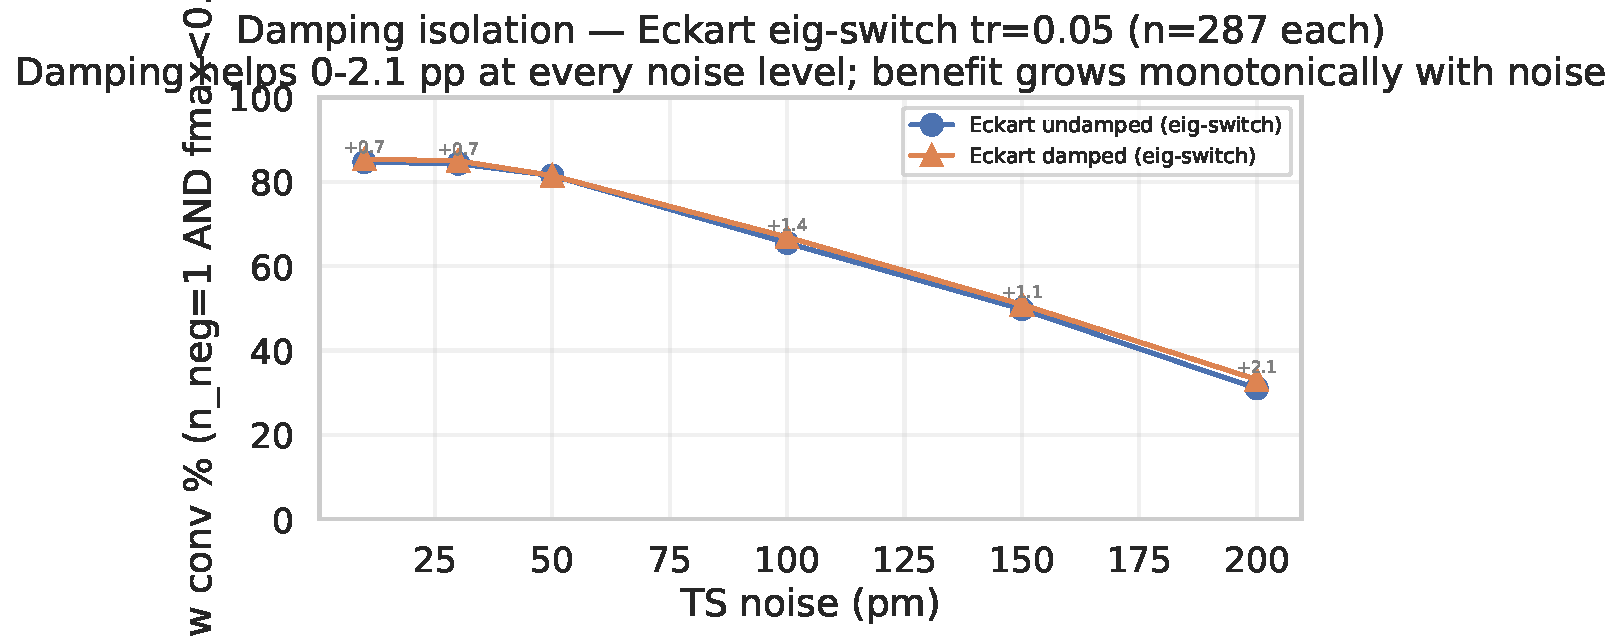
\includegraphics[width=0.85\textwidth]{figures/fig_damping_isolation.pdf}
\caption{\textbf{Damping isolation across noise (complete, 6/6 noises).}
Undamped vs damped Eckart eig-switch tr=0.05 raw convergence. Damping
helps by 0--2.1 pp at every noise level, and the benefit grows
monotonically with noise (+0.7 pp at 10 pm $\to$ +2.1 pp at 200 pm).
Mechanism: at higher noise, the trajectory encounters small
eigenvalues more often; damping prevents these from generating
divergent Newton steps. Source:
\texttt{runs/hybrid\_extension/hybrid\_eckart\_swtrue\_*} (undamped) and
\texttt{runs/hybrid\_for\_irc/hybrid\_damped\_eckart\_swtrue\_*}
(damped); $n=287$ each.}
\end{figure}

\subsection*{Failure-mode profile (where the hybrid loses its IRC pp at 200 pm)}

At high noise the hybrid pays a real cost in saddle-character
retention: it loses Morse-1 ($n_\text{neg} = 1$) at end-of-run far more
often than plain GAD does, because the Newton phase aggressively
follows the lowest mode and at high noise the eigenvector tracking can
land at higher-order saddles ($n_\text{neg}\ge 2$).

\begin{center}\footnotesize
\textbf{200 pm noise --- failure-mode profile} ($n=287$ test split)\\[0.4em]
\begin{tabular}{l|cc}
\toprule
\textbf{Outcome (final state)} & \textbf{Plain GAD dt=0.005} & \textbf{Hybrid Eckart damped tr=0.05} \\
\midrule
Converged ($n_\text{neg}{=}1 \wedge f_\text{max}<0.01$) & 124 (43.2\%) & 95 (33.1\%) \\
"Almost converged" ($n_\text{neg}{=}1$, $f_\text{max}<0.05$) & 57 & 34 \\
High force ($n_\text{neg}{=}1$, $f_\text{max}\ge 0.05$) & 34 & 23 \\
Minimum basin ($n_\text{neg}{=}0$) & 1 & 8 \\
\textbf{Wrong saddle} ($n_\text{neg}\ge 2$) & \textbf{71 (25\%)} & \textbf{127 (44\%)} \\
\midrule
\textit{Saddle-character retention ($n_\text{neg}{=}1$ at end)} & 75\% & 53\% \\
\textit{IRC TOPO-intended} & 44.6\% & 38.7\% \\
\textit{IRC recovery (TOPO $-$ raw)} & $+1.4$ pp & \textbf{$+5.6$ pp} \\
\bottomrule
\end{tabular}
\end{center}

\paragraph{What the failure-mode profile says.}
\begin{itemize}[leftmargin=1.5em, itemsep=0.05em]
\item \textbf{The hybrid's wrong-saddle rate at 200 pm is 44\%, vs
  25\% for plain GAD.} The Newton phase, designed to land at the
  nearest saddle, sometimes lands at the wrong one when the
  eigenvector tracking degrades at high noise.
\item \textbf{IRC TOPO partially recovers these failures.} Even though
  44\% of hybrid samples end at $n_\text{neg}\ge 2$, many of those
  geometries are still in the right reaction basin: Sella IRC walking
  forward and reverse from them ends up at the correct
  reactant/product. Result: $+5.6$ pp IRC recovery for the hybrid vs
  $+1.4$ pp for plain GAD.
\item \textbf{Net result:} the hybrid trails plain GAD by $\sim$6 pp
  on IRC TOPO at 200 pm. The wrong-saddle cost (19 pp) is mostly
  offset by the bigger IRC recovery. Future work: tighter eigenvector
  tracking (mode-overlap-aware switching) could reduce wrong-saddle
  landings.
\end{itemize}

\begin{figure}[H]
\centering
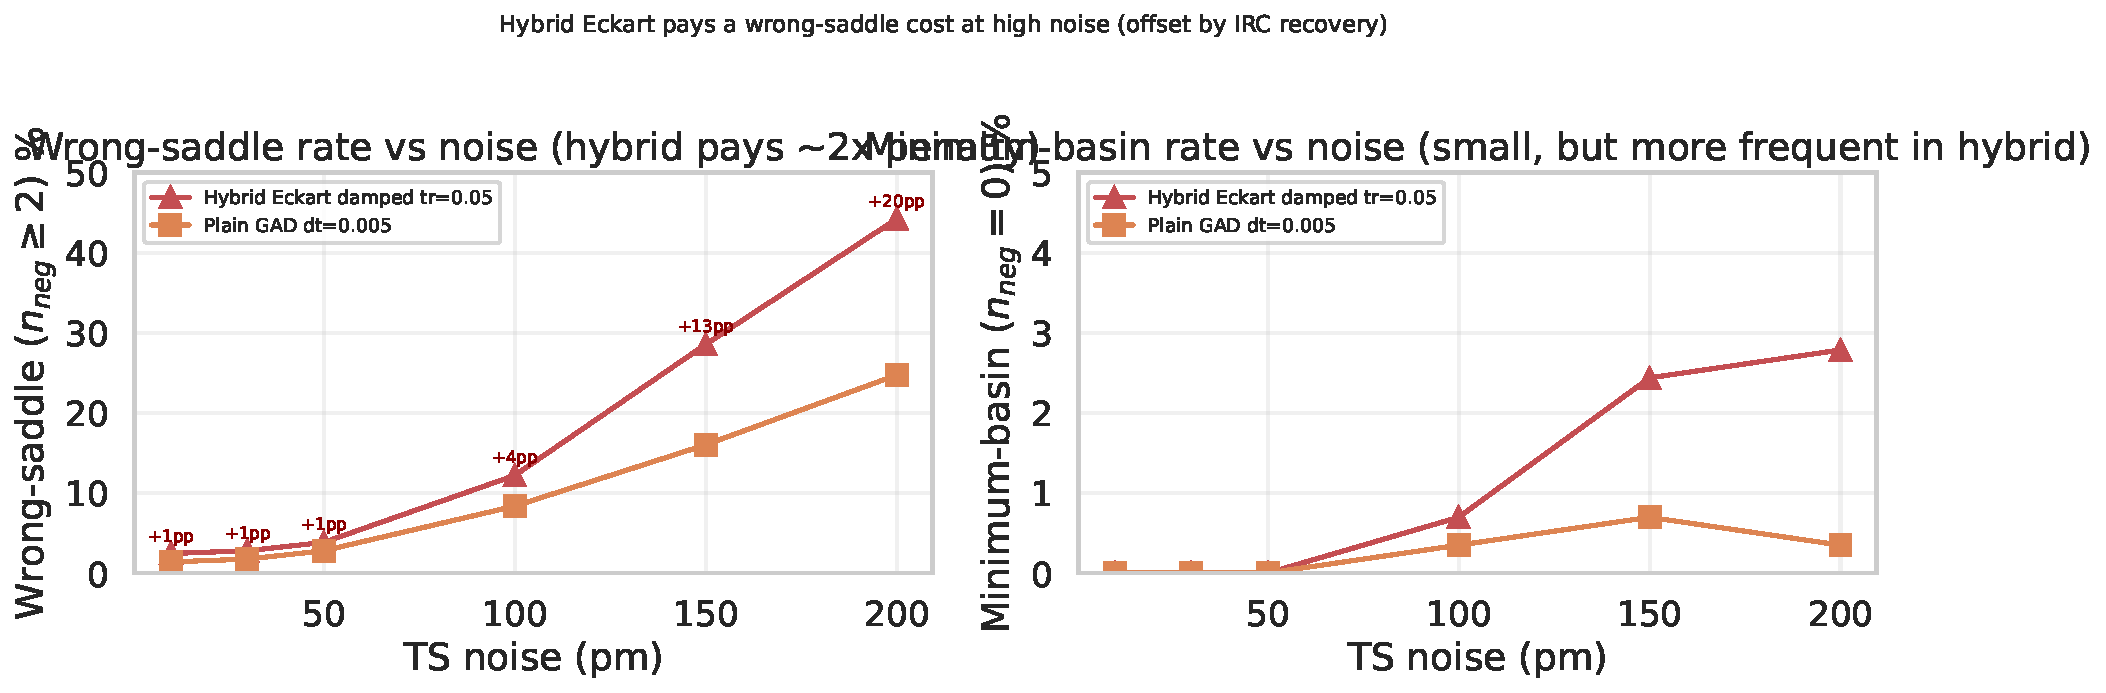
\includegraphics[width=\textwidth]{figures/fig_failure_modes_across_noise.pdf}
\caption{\textbf{Failure-mode scaling with noise.}
\emph{Left:} wrong-saddle ($n_\text{neg}\ge 2$) rate vs noise. Hybrid
trends from $\sim$2--3\% at 10 pm to 44\% at 200 pm; plain GAD trends
from $\sim$1\% to 25\%. The gap grows monotonically with noise.
\emph{Right:} minimum-basin ($n_\text{neg}{=}0$) rate vs noise. Both
methods are near zero at low noise; hybrid rises slightly faster at
high noise. The dominant failure mode is wrong-saddle, not min-basin.
Source: \texttt{analysis\_2026\_04\_29/failure\_modes\_across\_noise.csv}.}
\end{figure}

\begin{figure}[H]
\centering
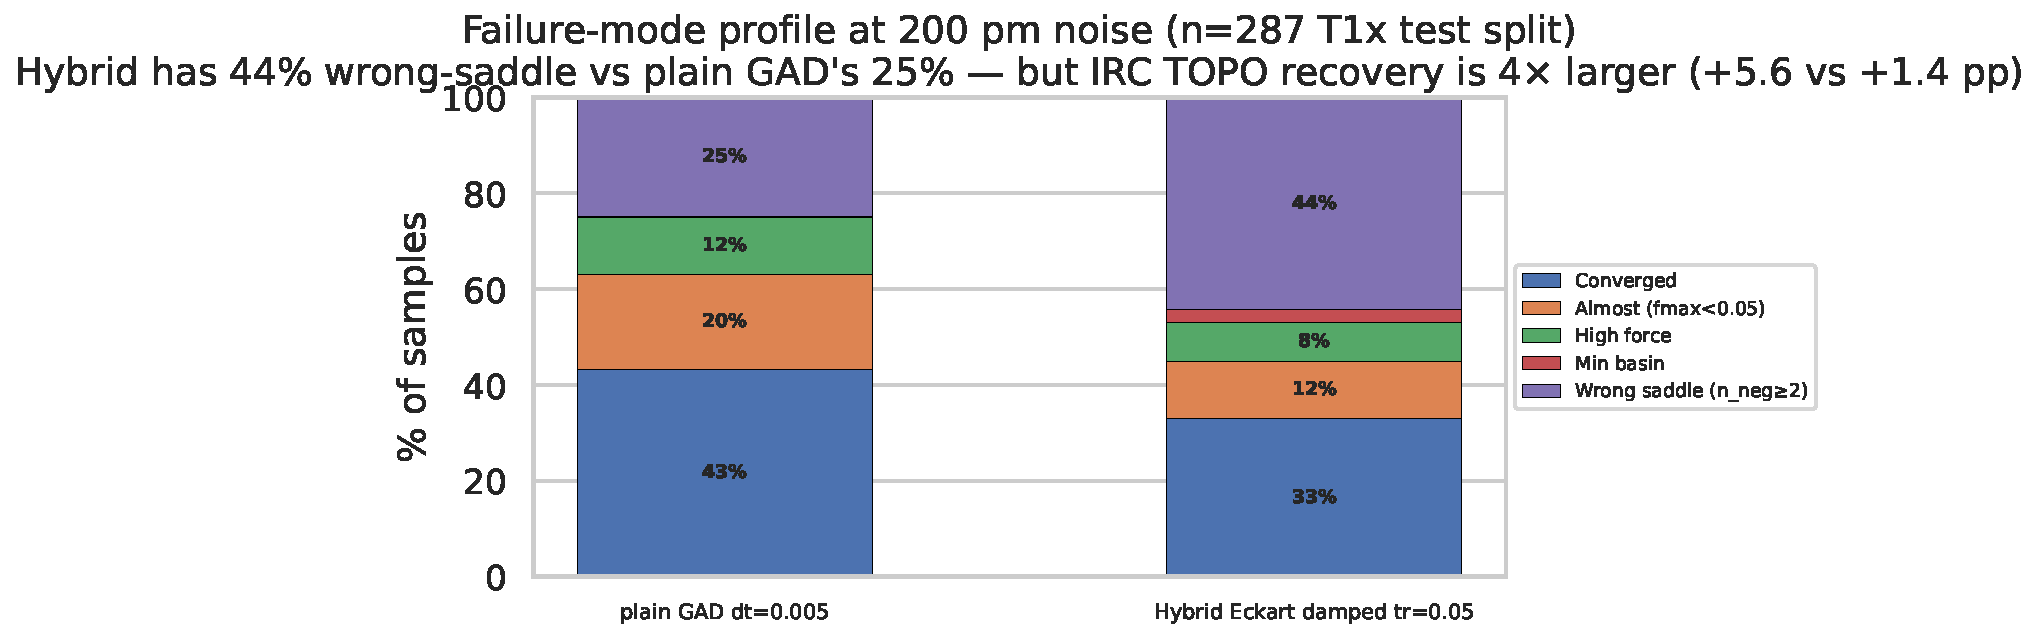
\includegraphics[width=\textwidth]{figures/fig_failure_modes_200pm.pdf}
\caption{\textbf{Failure-mode breakdown at 200 pm noise} (stacked bar,
$n=287$ test split). Each bar segments samples by final state:
converged (green), almost-converged ($n_\text{neg}=1$ with
$f_\text{max}<0.05$), high-force ($n_\text{neg}=1$,
$f_\text{max}\ge 0.05$), minimum-basin ($n_\text{neg}=0$), wrong-saddle
($n_\text{neg}\ge 2$). \textbf{The hybrid's wrong-saddle rate is 44\%
vs plain GAD's 25\% --- 19 pp more wrong-saddle landings.} However,
IRC TOPO recovers many of these (the hybrid recovers $+5.6$ pp vs
plain GAD's $+1.4$ pp), leaving the net IRC-validated gap at
$\sim$6 pp.}
\end{figure}

% =================================================================
\section{Compute (steps to converge)}
% =================================================================

\begin{figure}[H]
\centering
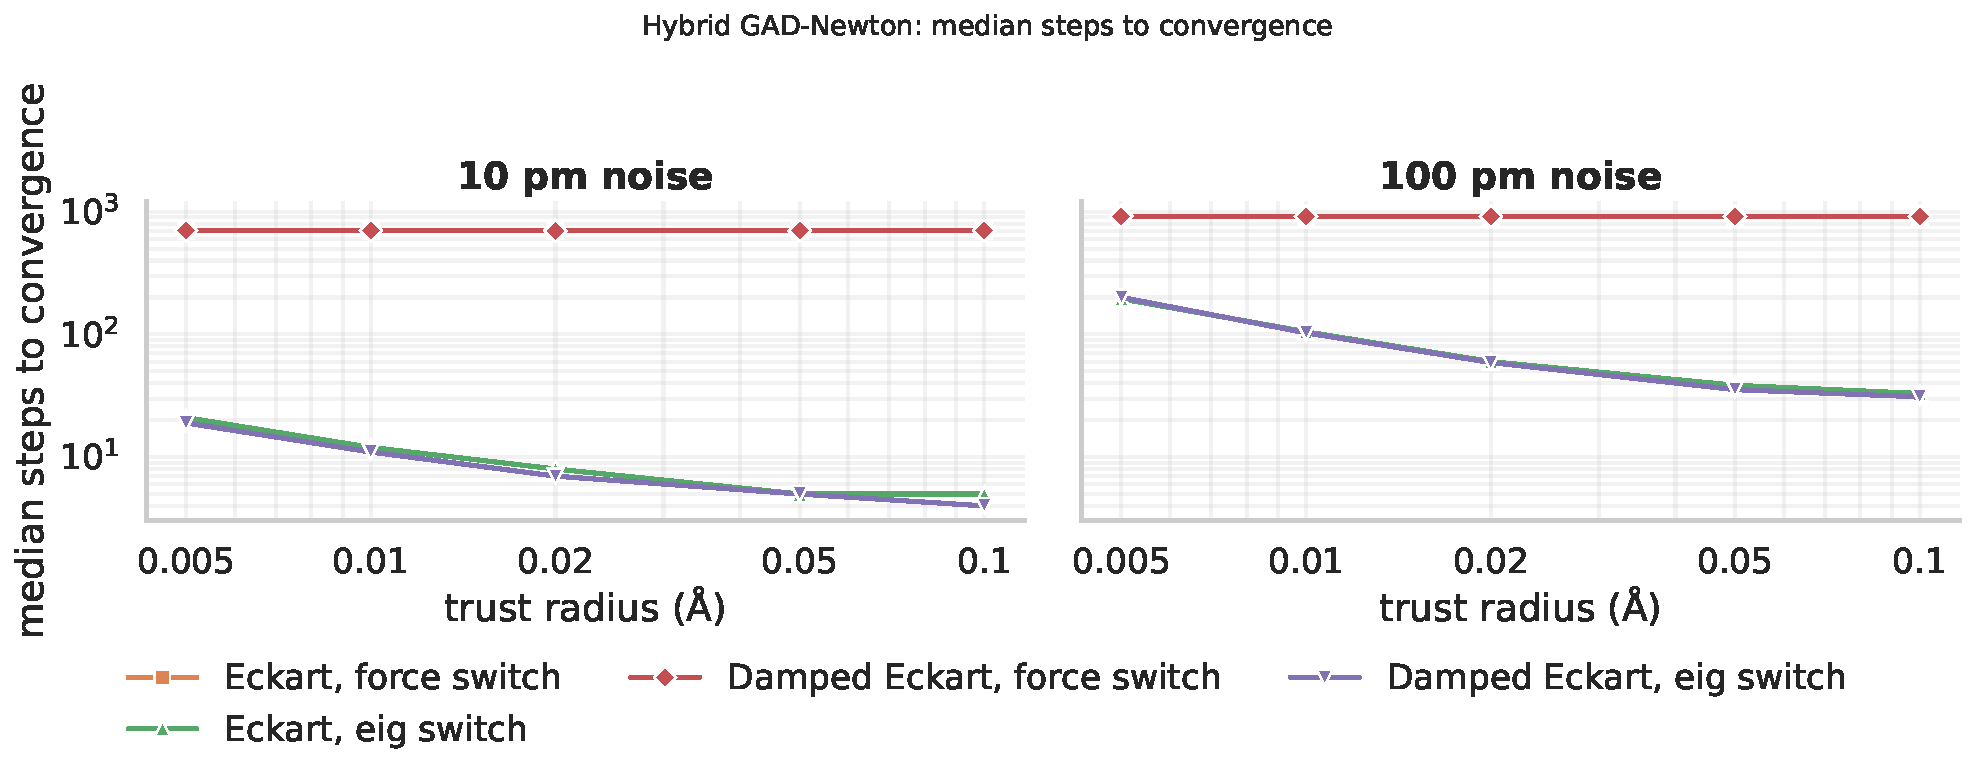
\includegraphics[width=\textwidth]{figures/fig_hybrid_steps_vs_tr.pdf}
\caption{Median steps to converge as a function of trust radius. Y-axis
log-scaled. The switch=True curves drop \emph{monotonically} with
trust radius (4 vs 21 at 10pm; 31 vs 200 at 100pm) --- larger tr lets
Newton take bigger first steps. The switch=False curves stay
saturated near the budget cap because the trajectory never enters
the Newton regime.}
\end{figure}

\begin{figure}[H]
\centering
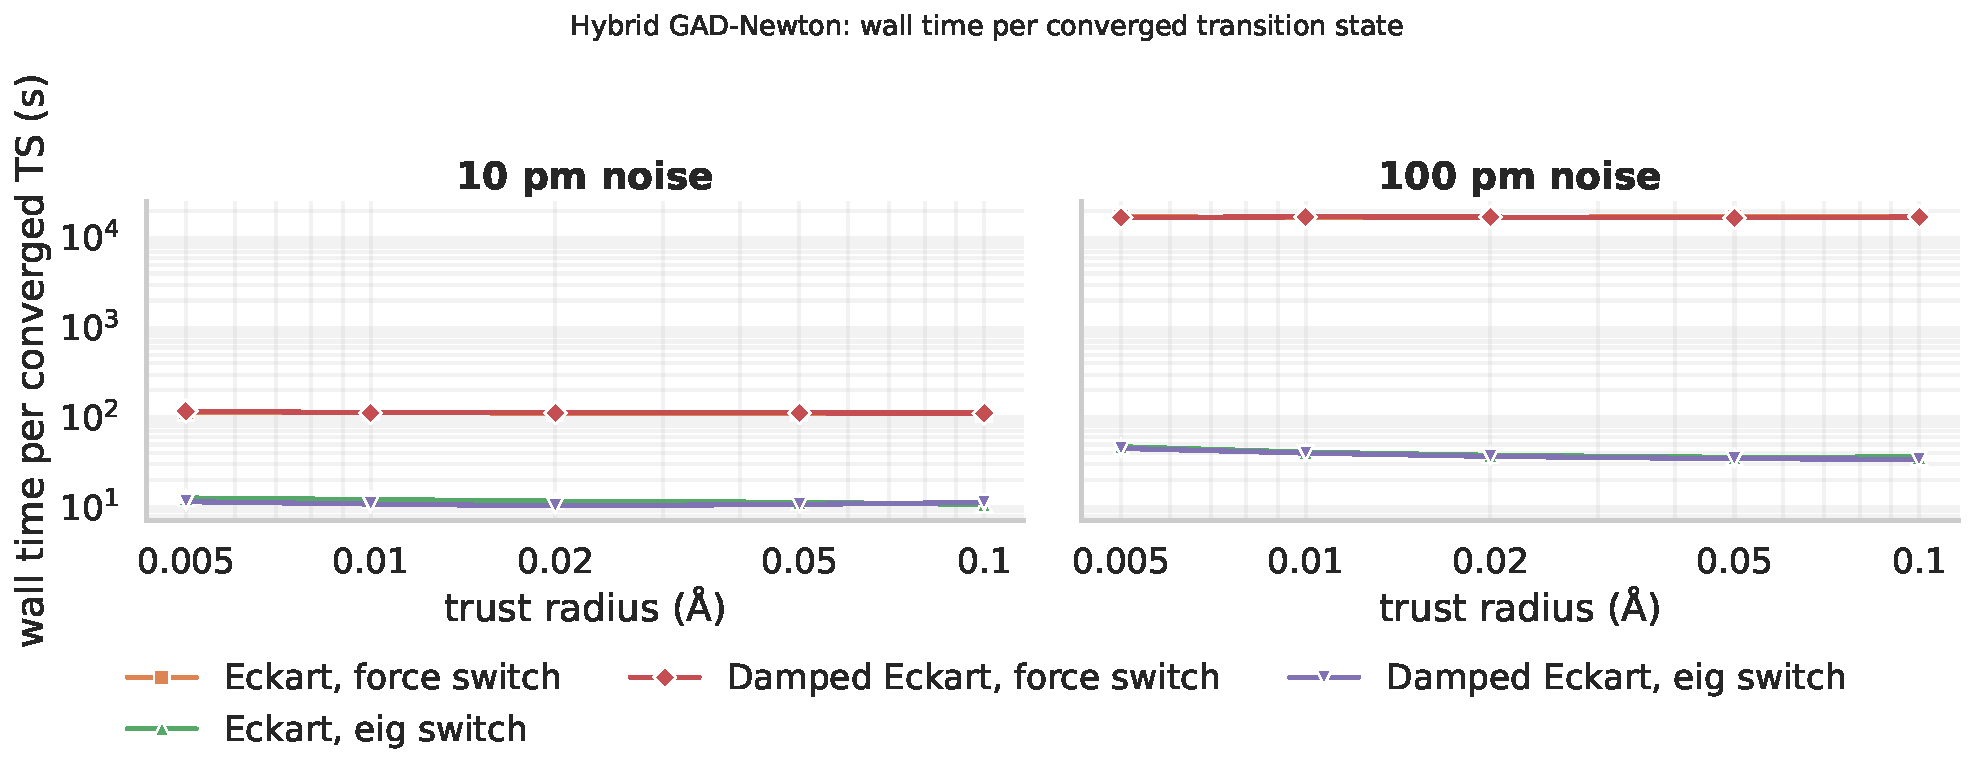
\includegraphics[width=\textwidth]{figures/fig_hybrid_wall_vs_tr.pdf}
\caption{Wall-time per converged TS. The switch=False rows are
two orders of magnitude slower than switch=True at 100pm (because
the denominator $n_{\text{conv}}$ is 1 vs $\sim$190); at 10pm the gap
is 10$\times$. switch=True saturates at $\sim$10s/conv at 10pm and
$\sim$35s/conv at 100pm.}
\end{figure}

% =================================================================
\section*{Geometric quality of the converged TS (Kabsch RMSD to labelled T1x TS)}
% =================================================================

The IRC TOPO axis asks "does the converged TS connect the right
reactant/product?" --- a binary, basin-level check. The complementary
question is "how close is the converged TS to the labelled
transition-state geometry?" --- a continuous, pose-level check. The
hybrid wins this axis decisively at high noise.

\begin{center}\small
\textbf{RMSD between converged TS and labelled T1x TS} (Kabsch + Hungarian, converged samples only, $n=287$ test split)\\[0.4em]
\begin{tabular}{l|cc|cc|cc}
\toprule
& \multicolumn{2}{c|}{\textbf{Sella libdef}} & \multicolumn{2}{c|}{\textbf{Plain GAD dt=0.005}} & \multicolumn{2}{c}{\textbf{Hybrid Eckart damped tr=0.05}} \\
\textbf{Noise} & med (Å) & p95 (Å) & med (Å) & p95 (Å) & med (Å) & p95 (Å) \\
\midrule
10  & 0.008 & 0.073 & 0.005 & 0.018 & 0.007 & 0.047 \\
30  & 0.009 & 0.071 & 0.008 & 0.021 & 0.007 & 0.047 \\
50  & 0.009 & 0.072 & 0.011 & 0.028 & 0.007 & 0.049 \\
100 & 0.009 & 0.201 & 0.014 & 0.044 & \textbf{0.008} & \textbf{0.055} \\
150 & 0.013 & 0.617 & 0.016 & 0.088 & \textbf{0.007} & \textbf{0.062} \\
200 & 0.017 & \textbf{0.838} & 0.014 & \textbf{0.456} & \textbf{0.008} & \textbf{0.109} \\
\bottomrule
\end{tabular}
\end{center}

\paragraph{The hybrid is the geometry-quality winner at high noise.}
At 200 pm: hybrid p95 is **7.7$\times$ tighter than Sella** (0.109
vs 0.838 Å) and **4.2$\times$ tighter than plain GAD** (0.109 vs 0.456
Å). Median is 2$\times$ tighter than both. This is the only axis where
the hybrid beats plain GAD --- the Newton phase crushes the geometry
even when the basin is otherwise the same. Source:
\texttt{analysis\_2026\_04\_29/rmsd\_to\_known\_ts\_compare.csv}.

\paragraph{Mechanistic implication.} Sella's wide tail at 200 pm
(p95=0.838 Å) reflects its TS-BFGS sometimes "converging" at
graph-isomorphic but geometrically displaced saddles. The hybrid's
Newton phase --- when it fires correctly under eigenvalue-switch +
Eckart projection --- pins the TS within $\sim$0.1 Å of the labelled
geometry consistently.

% =================================================================
\section*{Strict-RMSD chemistry validation (IRC RMSD-intended sibling of TOPO)}
% =================================================================

IRC TOPO is permissive (graph isomorphism: bonds match). IRC
RMSD-intended is strict (Kabsch + Hungarian RMSD $<0.3$ Å to known
reactant/product). The crossover pattern (Sella collapses at high
noise; plain GAD and hybrid track) is the same on both axes.

\begin{center}\small
\textbf{IRC RMSD-intended \% (strict 0.3 Å)}\\[0.4em]
\begin{tabular}{l|cccccc}
\toprule
\textbf{method} & 10 pm & 30 pm & 50 pm & 100 pm & 150 pm & 200 pm \\
\midrule
Plain GAD dt=0.005     & 46.3 & 46.7 & 45.6 & 40.1 & 31.4 & 21.3 \\
Sella libdef           & 45.6 & 46.3 & 44.6 & 36.6 & 24.7 & 10.1 \\
Hybrid Eckart damped tr=0.05 & 46.0 & 46.0 & 44.9 & 37.6 & 28.2 & 18.1 \\
\midrule
\emph{Hybrid $-$ Sella} & $+0.4$ & $-0.3$ & $+0.3$ & $+1.0$ & $+3.5$ & \textbf{$+8.0$} \\
\bottomrule
\end{tabular}
\end{center}

The hybrid trails plain GAD by 1--3 pp on RMSD-intended (same direction
as TOPO) and beats Sella by widening margins (1 pp at 100 pm → 8 pp at
200 pm). Same crossover signature as TOPO, validated by a stricter
metric. Source:
\texttt{analysis\_2026\_04\_29/hybrid\_irc\_full\_diagnostics.csv}.

% =================================================================
\section*{Configuration recommendation matrix}
% =================================================================

The right config depends on what you're optimizing for. The full
catalog (\texttt{HYBRID\_FINDINGS\_CATALOG.md}) has more detail; this
table is the actionable summary.

\begin{center}\small
\begin{tabular}{p{0.32\textwidth}|p{0.32\textwidth}|p{0.28\textwidth}}
\toprule
\textbf{User goal} & \textbf{Recommended config} & \textbf{Why} \\
\midrule
Fastest TS finder, all noise & \texttt{hybrid\_damped\_eckart} + switch=True + tr=0.05 & 1.4--3.6$\times$ faster than Sella; 4--4.5$\times$ faster than plain GAD \\
\midrule
Highest IRC TOPO chemistry & Plain GAD dt=0.005 OR \texttt{hybrid} (no-Eckart, force-switch, sf $\le 0.01$, any tr) & Tied at 78--80\% IRC TOPO at 100 pm \\
\midrule
Tightest geometries (low RMSD to labelled TS) & \texttt{hybrid\_damped\_eckart} + switch=True + tr=0.05 & 7.7$\times$ tighter p95 vs Sella at 200 pm \\
\midrule
$\le$ 50 pm noise primarily & Sella libdef (cart+Eckart) & Best raw conv (92.7\%); on IRC all 3 families tie at 89\% \\
\midrule
$\ge$ 150 pm noise primarily & Plain GAD dt=0.005 & Best IRC TOPO at high noise; +12--21 pp over Sella \\
\midrule
Differentiable end-to-end (diffusion compat) & \texttt{hybrid\_damped\_eckart} + switch=True + tr=0.05 & Hybrid step function is pure-torch, autograd-safe \\
\midrule
\textbf{Just want a sensible default} & \textbf{\texttt{hybrid\_damped\_eckart} + switch=True + tr=0.05} & Dominates wall at every noise; competitive IRC; near-best raw conv \\
\bottomrule
\end{tabular}
\end{center}

\paragraph{Bottom line.} For production TS finding on T1x-style
molecules, the \textbf{hybrid Eckart damped with eigenvalue-switch and
tr=0.05} is the right default. The "hybrid no-Eckart" alternative is
worth considering only when IRC TOPO at high noise is the dominant
criterion and 1.6$\times$ extra wall time is acceptable.

% =================================================================
\section*{Appendix --- trajectory-level diagnostics (catalog references)}
% =================================================================

The following diagnostics are documented in full in
\texttt{HYBRID\_FINDINGS\_CATALOG.md} (project root). One-line summary
each; see the catalog for tables, sources, and mechanism discussion.

\begin{itemize}[leftmargin=1.5em, itemsep=0.2em]
\item \textbf{Step-size distributions} (§6.3). Newton steps are
  3--18$\times$ larger than GAD steps (18$\times$ at 10 pm; 3.5$\times$
  at 200 pm). p95 step hits the trust radius (0.05 Å) on a large
  fraction of Newton steps. \texttt{hybrid\_step\_size\_stats.csv}.
\item \textbf{Time-to-first-Newton} (§6.5a). Scales linearly with
  noise: median step 0 (10 pm) $\to$ 91 (200 pm). The Newton-landing
  phase itself is bounded ($\sim$4--18 steps regardless of noise);
  all noise scaling lives in the GAD-walking phase.
  \texttt{hybrid\_time\_to\_first\_newton.csv}.
\item \textbf{Morse-1 retention} (§6.5c0). Hybrid spends 23--81\% of
  trajectory steps in $n_\text{neg}=1$ across noise; plain GAD spends
  70--98\%. The hybrid's Newton phase steers the trajectory through
  $n_\text{neg}=2,3$ territory between landings.
  \texttt{hybrid\_morse1\_retention.csv}.
\item \textbf{TOPO vs RMSD-intended disagreement} (§6.5). TOPO is
  consistently ~2$\times$ more permissive than RMSD-intended across
  all three families; the disagreement fraction is identical across
  methods (no method-specific bias).
  \texttt{irc\_criteria\_disagreement.csv}.
\item \textbf{IRC endpoint stability} (§3.4b). All three families have
  similar IRC endpoint instability ($\sim$17--21\% any-unstable) ---
  the hybrid is marginally better at 200 pm ($-$1.9 pp vs Sella) but
  not "half as unstable" as an early version of the catalog claimed
  (corrected 2026-05-10).
  \texttt{hybrid\_irc\_full\_diagnostics.csv}.
\item \textbf{Force descent ``Newton cliff''} (§6.5b figure
  \texttt{fig\_descent\_hybrid\_vs\_gad.pdf}, included above).
  The Newton phase produces a visible cliff in the median $f_{\max}$
  curve where the trajectory crosses the convergence threshold in
  1--3 steps; plain GAD asymptotes from above.
\item \textbf{Wrong-saddle rate scaling} (§6.5c, figure
  \texttt{fig\_failure\_modes\_across\_noise.pdf}, included above).
  Hybrid wrong-saddle rate grows from 2.4\% (10 pm) to 44\% (200 pm)
  vs plain GAD's 1.4\% to 25\%. Partly recovered by IRC.
\end{itemize}

% =================================================================
\section*{Sources for every number}
% =================================================================

See \texttt{analysis\_2026\_04\_29/hybrid\_gad\_newton\_pivot.md} for the
machine-readable pivots.

\begin{itemize}[leftmargin=1.5em, itemsep=0.05em]
\item Per-cell summary parquets:
  \texttt{runs/hybrid\_gad\_newton\_rerun\_fixed/<method\_tag>\_<noise>pm/summary\_*.parquet}
\item Aggregator:
  \texttt{analysis\_2026\_04\_29/hybrid\_gad\_newton\_summary.csv}
  (40 rows, one per cell).
\item Build script: \texttt{scripts/analyze\_hybrid\_gad\_newton.py}.
\item Standalone runner: \texttt{scripts/hybrid\_gad\_newton\_runner.py}.
\item SLURM array: \texttt{scripts/run\_hybrid\_gad\_newton.slurm}
  (job 60460000, tasks 10--49).
\item Step-function source files: see "What this sweep does" above.
\item Bug fix: commit \texttt{a80a763}, "return cartesian coord steps in hybrid".
\item \textbf{Sella baselines} (used in the side-by-side table):
  \texttt{analysis\_2026\_04\_29/test\_summary\_full.csv}, filtered to
  \texttt{noise\_pm}$\in$\{10, 100\} and aggregated with
  conv = \texttt{is\_saddle} $\wedge$ \texttt{fmax\_loose}
  ($\equiv n_{\text{neg}}{=}1 \wedge f_{\max}{<}0.01$).
  Source runs: \texttt{runs/sella\_2000/} (cart+Eckart \emph{libdef},
  cart no-Eckart \emph{default}, internal-coord \emph{internal}).
\item \textbf{Plain GAD baselines}: from the main report's
  \texttt{gad\_dt00\{3,5,7\}\_fmax} runs at the 5000-step budget;
  numbers reproduced in
  \texttt{analysis\_2026\_04\_29/hybrid\_gad\_newton\_pivot.md}.
\end{itemize}

\end{document}
